\documentclass[10pt, a4paper, cleardoubleempty, openright, twoside]{book}
%%%%%%%%%%%%%%%%%%%%%%%%%%%%%%
%%% Packages & Definitions %%%
%%%%%%%%%%%%%%%%%%%%%%%%%%%%%%

\usepackage[T1]{fontenc}
\usepackage[latin1]{inputenc}

\usepackage{amsmath,amsfonts,amssymb,dsfont,amsxtra,amsopn,amstext,amsbsy}

\usepackage[rightcaption]{sidecap}
\usepackage[hang]{caption2}
\usepackage{mycap}

\usepackage[]{tocbibind}
\usepackage{epigraph}
\usepackage{csquotes}
\usepackage{fancyhdr,fancybox}

\usepackage[english]{babel}

\usepackage{graphicx}
\usepackage[dvips]{rotating}
\usepackage{color}
\definecolor{violet}{cmyk}{0.94,0.86, 0.04,0.08}

\usepackage[
colorlinks, % Schrift in Farbe, sonst mit Rahmen
linktocpage, % stellt mein Inhaltsverzeichnis richtig dar
bookmarksnumbered, % Inhaltsverzeichnis mit Numerierung
bookmarksopen, % ^?offnet das Inhaltsverzeichnis
pdfstartview=FitH, % startet mit Seitenbreite
linkcolor=blue, % standard red
citecolor=blue, % standard green
urlcolor=violet, % standard cyan
filecolor=blue %
backref % man kommt von der bibo zurueck
]{hyperref}
\usepackage{makeidx}

\makeindex

\graphicspath{{figures/}}
%%%%%%%%%%%%%%%%%%%%%%%%%%%%%%%%%
%%% Correction Style Commands %%%
%%%%%%%%%%%%%%%%%%%%%%%%%%%%%%%%%

\newcommand{\marginlabel}[1]{\mbox{}\marginpar{\raggedright\hspace{0pt}\emph{#1}}}
\newcommand{\bs}[1]{{\color{red}{XXX}}\marginlabel{#1}}
\newcommand{\new}[1]{{\color{red}{#1}}\marginlabel{ADDED}}
\newcommand{\zitat}{[\color{red}\textbf{Zitat}]\marginlabel{Zitat} }
\newcommand{\zitate}[1]{{\color{red}{[\textbf{#1}]}}\marginlabel{Zitat} }

%%%%%%%%%%%%%%%%%%%%%%
%%% Epigraph Style %%%
%%%%%%%%%%%%%%%%%%%%%%
\setlength\epigraphwidth{12cm}
%\setlength\epigraphrule{0pt}


%%%%%%%%%%%%%%%%%%%%%%%%%%%
%%% Page Style Commands %%%
%%%%%%%%%%%%%%%%%%%%%%%%%%%

\setlength{\hoffset}{-1in}
\setlength{\voffset}{-1in}
\setlength{\textwidth}{14.5cm}
\setlength{\textheight}{22.2cm}
\setlength{\evensidemargin}{3cm}
\setlength{\oddsidemargin}{3.5cm}
\setlength{\marginparwidth}{2.0cm}
\setlength{\marginparsep}{0.5cm}
\setlength{\topmargin}{2.0cm}
\setlength{\headheight}{1cm}
\setlength{\topskip}{0.5cm}
\setlength{\footskip}{1.0cm}

\setcounter{secnumdepth}{1}
\setcounter{tocdepth}{1}

%%%%%%%%%%%%%%%%%%%%%
%%% Caption style %%%
%%%%%%%%%%%%%%%%%%%%%

\setboolean{capbreak}{false}
\renewcommand{\capshape}{}
\renewcommand{\capfont}[1]{\tc{\textsf{#1}}}
\renewcommand{\fnumfont}[1]{\tc{\textbf{\textsf{#1}}}}
%\renewcommand{\fnumshape}[1]{\rule{\linewidth}{1pt}\\ #1 | }
\renewcommand{\fnumshape}[1]{#1 | }

%%%%%%%%%%%%%%%%%%%%%
%%% Section style %%%
%%%%%%%%%%%%%%%%%%%%%

\makeatletter
\renewcommand{\subsubsection}{\@startsection%
	{subsubsection}%
	{3}%
	{1em}%
	{\baselineskip}%
	{-\fontdimen2\font plus -\fontdimen3\font minus -\fontdimen4\font}%
	{\normalfont\bfseries}
}%
\makeatother

\newcommand{\tc}[1]{\textcolor{violet}{#1}}

\newcommand{\np}{\newpage}
\newcommand{\cp}{\clearpage}


%
%%
%%%
%%%%%%%%%%%%
%%% Main %%%
%%%%%%%%%%%%
%%%
%%
%




\begin {document}

\frontmatter
%%%%%%%%%%%%%%%%%%%%%%%
%%% title & abstract %%
%%%%%%%%%%%%%%%%%%%%%%%
\pagestyle{empty}


	\begin{figure}[h!]
		\begin{center}
			
\includegraphics[width=0.5\textwidth]{figures/logo}
		\end{center}
	\end{figure}

	\vfill 

\begin{center}
	\begin{Huge}
		THE ZEITGEIST MOVEMENT DEFINED
	\end{Huge}

	\vfill

	\begin{LARGE}
		REALIZING A NEW TRAIN OF THOUGHT
	\end{LARGE}

	\vfill 

	\begin{quote}
	\begin{itshape}
		The tremendous and still accelerating development of science and
		technology has not been accompanied by an equal development in
		social, economic, and political patterns... We are now ... only
		beginning to explore the potentialities which it offers for
		developments in our culture outside technology, particularly in the
		social, political and economic fields. It is safe to predict that
		... such social inventions as modern-type Capitalism, Fascism, and
		Communism will be regarded as primitive experiments directed toward
		the adjustment of modern society to modern technology.\\
	\end{itshape}
		-- Dr. Ralph Linton
	\end{quote}

	\vfill 

	www.thezeitgeistmovement.com

\end{center}

\cleardoublepage


\pagestyle{fancy}

%%%%%%%%%%%%%%%%%%%%%%
%%% Fancy Headings %%%
%%%%%%%%%%%%%%%%%%%%%%
\renewcommand{\headrulewidth}{0.5pt}
\renewcommand{\footrulewidth}{0.5pt}

\fancyhead{}
\renewcommand{\chaptermark}[1] {
	\fancyhead[LO]{}
	\fancyhead[RE]{\sc\thechapter\space#1}
}
\renewcommand{\sectionmark}[1]{
		\fancyhead[LO]{\sc\thesection\space#1}
	}
\fancyfoot{}
\fancyfoot[RO,LE]{\small\thepage}

\fancypagestyle{plain} {
	\fancyhead{}
	\renewcommand{\headrulewidth}{0pt}
	\fancyfoot{}
	\fancyfoot[RO,LE]{\thepage}
}

\fancypagestyle{empty} {
	\fancyhead{}
	\renewcommand{\headrulewidth}{0pt}
	\renewcommand{\footrulewidth}{0pt}
	\fancyfoot{}
}

\setcounter{page}{1}% \pagenumbering{roman}
\pagestyle{fancy}

\tableofcontents
\listoffigures
\listoftables
\cleardoublepage

\chapter {Preface}
\epigraph{\itshape
	The outcome of any serious research can only be to make two questions
	grow where only one grew before.
}{Thorstein Veblen~\cite{Veblen:UCC:08}}

\addcontentsline{toc}{section}{Origin of the name}
\section* {Origin of the name}

\emph{\textquote{The Zeitgeist Movement}} (TZM) is the identifier for
the social movement described in the following essays. The name has no
relevant historical reference to anything culturally specific and is not
to be confused or associated with anything else known before with a
similar title. Rather, the title is based upon the semantic meaning of
the very terms, explicitly.

The term \emph{zeitgeist} is defined as the \emph{general intellectual,
moral and cultural climate of an era.} The term \emph{movement} simply
implies \emph{motion} or change. Therefore, The Zeitgeist Movement is an
organization that urges change in the dominant intellectual, moral and
cultural climate of the time.

\addcontentsline{toc}{section}{Document Structure}
\section* {Document Structure}
The following text has been prepared to be as concise and yet
comprehensive as possible. In form, it is a series of essays, ordered by
subject in a manner that works to support a broader \emph{context}.
While each essay is designed to be taken on its own merit in evaluation,
the true context resides in how each issue works to support a larger
\emph{train of thought} with respect to the most efficient organization
of human society.

It will be noticed by those who read through these essays in a linear
fashion that a fair amount of overlap exists with certain ideas or
subjects. This is deliberate as such repetition and emphasis is
considered helpful given how foreign some of the concepts might seem to
those with no prior exposure to such material.

Also, since only so much detail can be afforded to maintain
comprehension given the gravity of each subject and how they
interrelate, great effort has been made to source relevant third party
research throughout each essay via footnotes, allowing the reader to
follow through with further study as the interest arises.

\addcontentsline{toc}{section}{The Organism of Knowledge}
\section* {The Organism of Knowledge}
As with any form of presented research we are dealing with
\emph{serially generated data composites}. Observation, its assessment,
documentation and integration with other knowledge, existing or pending,
is the manner by which all distinguishable ideas come to evolve.

This continuum is important to understand with respect to the way we
think about what we believe and why, for information is always separate
in its merit from the person or institution communicating or
representing. Information can only be evaluated correctly through a
systematic process of comparison to other \emph{physically verifiable}
evidence as to its proof or lack thereof.

Likewise, this continuum also implies that there can be no empirical
\textquote{origin} of ideas. From an epistemological perspective,
knowledge is mostly culminated, processed and expanded through
communication amongst our species. The individual, with his or her
inherently different life experience and propensities, serves as a
custom-processing \emph{filter} by which a given idea can be morphed.
Collectively, we individuals comprise what could be called a \emph{group
mind}, which is the larger order social processor by which the efforts
of individuals ideally coalesce. The traditional method of data transfer
through literature, sharing books from generation to generation, has
been a notable path of this group mind interaction, for
example.\footnote{
	In Carl Sagan's work \textquote{Cosmos}, he stated with respect to the
	destruction of the Library of Alexandria, noted as the largest and
	most significant library of the ancient world: \blockcquote[ch.~XIII,
	p.~279]{Sagan::80}{It was as if the entire civilization had undergone
	some self-inflicted brain surgery, and most of its memories,
	discoveries, ideas and passions were extinguished irrevocably.}
}

Isaac Newton perhaps put this reality best with the statement:
\blockcquote[p.~416]{Turnbull::59}{If I have seen further than others,
it is by standing upon the shoulders of giants.} This is brought up here
in order to focus the reader on the critical consideration of data, not
a supposed \textquote{source}, as there actually is no such thing in an
empirical sense. It is only in the temporal, traditional patterns of
culture, such as with literary credits in a textbook for future research
reference, is such a recognition technically relevant.

There is no statement more erroneous than the declaration that
\textquote{this is my idea}. Such notions are byproducts of a material
culture that has been reinforced in seeking physical rewards, usually
via money, in exchange for the illusion of their \textquote{proprietary}
creations. Very often an ego association is culminated as well where an
individual claims prestige about their \textquote{credit} for an idea or
invention.

Yet, that is not to exclude gratitude and respect for those figures or
institutions that have shown dedication and perseverance towards the
expansion of knowledge itself, nor to diminish the necessity of
importance of those who have achieved a skilled, specialized
\textquote{expert} status in a particular field. The contributions of
brilliant thinkers and engineers such as R. Buckminster Fuller, Jacque
Fresco, Jeremy Rifkin, Ray Kurzweil, Robert Sapolsky, Thorstein Veblen,
Richard Wilkinson, James Gilligan, Carl Sagan, Nikola Tesla, Stephen
Hawking and many, many more researchers, past and present, are quoted
and sourced in this text and serve as part of the larger \emph{data
composite} you are about to read. Great gratitude is also expressed here
towards all dedicated minds that are working to contribute to an
improving world.

That understood, \textquote{The Zeitgeist Movement} claims no
origination of any idea it promotes and is best categorized as an
activist/educational institution that works to amplify a \emph{context}
upon which existing/emerging scientific findings may find a concerted
social imperative.


\addcontentsline{toc}{section}{Websites and Resources}
\section* {Websites and Resources}
The following 10 websites are officially related to The Zeitgeist
Movement's global operations:

\begin{itemize}
	\item Main Global Hub:

	\url{http://www.thezeitgeistmovement.com}

	This is the main website and hub for TZM related
	actions/events/updates.

	\item Global Chapters Hub:
	
	\url{http://www.tzmchapters.net/}
	
	This is the main global hub for chapter information and materials. It
	includes maps, a chapter's tool kit and more.

	\item Global Blog:

	\url{http://blog.thezeitgeistmovement.com/}
	
	This is the official blog which allows submissions of editorial style
	essays.

	\item Global Forum:
	
	\url{http://www.thezeitgeistmovementforum.org/}
	
	This is the official forum for members to discuss projects and share
	ideas from across the world.

	\item Zeitgeist Media Project:
	
	\url{http://zeitgeistmediaproject.com/}
	
	The Media Project website hosts and links to various
	audio/visual/literary expressions create by TZM members. Users donate
	their work for posting and it is often used as a resource
	\emph{toolkit} for flyer graphics, video presentations, logo
	animations and the like.
	
	\item ZeitNews:
	
	\url{http://www.zeitnews.org/}
	
	ZeitNews is a news style service that contains articles relating to
	socially relevant advancements in science and Technology.

	\item Zeitgeist Day (\textquote{ZDay}) Global:

	\url{http://zdayglobal.org/}
	
	This site becomes active annually to facilitate our \textquote{Zday}
	global event, which occurs in March of each year.

	\item Zeitgeist Media Festival:
	
	\url{http://zeitgeistmediafestival.org/}
	
	This site becomes active annually to facilitate our
	\textquote{Zeitgeist Media Festival}, which occurs in autumn of each
	year.

	\item Global Redesign Institute:
	
	\url{http://www.globalredesigninstitute.org/}
	
	The Global Redesign Institute is a virtual graphic interface
	\textquote{think tank} project which uses map/data models to express
	direct technical changes in line with TZM's train of thought in
	various regions.
\end{itemize}

\addcontentsline{toc}{section}{General Social Networks}
\section* {General Social Networks}

\begin{itemize}
	\item TZM Global on Twitter:
	
	\url{http://twitter.com/#!/tzmglobal}

	\item TZM Global on Facebook:
	
	\url{http://www.facebook.com/tzmglobal}
	
	\item TZM Global Youtube:
	
	\url{http://www.youtube.com/user/TZMOfficialChannel}
\end{itemize}



\mainmatter



\part {Introduction}

\chapter {Overview}
\epigraph{\itshape
	Neither the great political and financial power structures of the
	world, nor the specialization-blinded professionals, nor the
	population in general realize that... it is now highly feasible to
	take care of everybody on earth at a \textquote{higher standard of
	living than any have ever known}. It no longer has to be you or me.
	Selfishness is unnecessary and henceforth unrationalizable as mandated
	by survival.  War is obsolete. 
}{R. Buckminster Fuller~\cite[Introduction, p.~xxv]{Fuller::81}}

\section {About}

Founded in 2008, The Zeitgeist Movement (TZM) is a sustainability
advocacy group that operates through a network of regional chapters,
project teams, public events, media expressions and charity operations.
TZM's activism is explicitly based on \emph{non-violent} methods of
communication with the core focus on \emph{educating} the public about
the true \emph{root sources} of many common personal, social and
ecological problems today, coupled with the vast \emph{problem solving}
and \emph{humanity improving potential} science and technology has now
enabled, but yet goes unapplied due to barriers inherent in the current,
established social system.

While the term \textquote{activism} is correct by its exact meaning,
TZM's awareness work should not be misconstrued as relating to
culturally common, traditional \textquote{activist protest} actions such
as we have seen historically. Rather, TZM expresses itself through
targeted, rational educational projects that work not to impose, dictate
or blindly persuade, but to set in motion a \emph{train of thought} that
is \emph{logically self-realizing} when the causal considerations of
\textquote{sustainability}\footnote{
	The term \textquote{sustainability}, generally defined \textquote{as
	the ability to be sustained, supported, upheld, or confirmed}
	(\url{http://dictionary.reference.com/browse/sustainability}) is often
	today commonly referenced/understood within an environmental science
	context. TZM's context extends farther, however, including the notion
	of cultural or behavioral sustainability, which considers the merit of
	belief systems in general, and their less obvious causal consequences.
}
and \textquote{public health}\footnote{
	The term \textquote{public health}, generally defined as
	\blockquote{the science and practice of protecting and improving the
	health of a community, as by preventive medicine, health education,
	control of communicable diseases, application of sanitary measures,
	and monitoring of environmental hazards}
	(\url{http://dictionary.reference.com/browse/public+health?s=t}) is
	used in this text as a basis of measure for the physical,
	psychological and hence sociological well-being of a societies' people
	over time. This is to be considered the ultimate barometer of the
	success or failure of an applied social system.
}
are referenced from a scientific perspective.

However, TZM's pursuit is still very similar to traditional civil rights
movements of the past in that the observations reveal the truly
unnecessary \emph{oppression} inherent in our current social order,
which structurally and sociologically restricts human well-being and
potential for the vast majority of the world's population, not to
mention stifles broad improvement in general due to its established
methods. 
	
For instance, the current social model, while perpetuating enormous
levels of corrosive economic inefficiency in general, as will be
described in further essays, also intrinsically supports one economic
group or \textquote{class} of people over another, perpetuating
technically unnecessary imbalance and high relative deprivation. This
could be called \textquote{economic bigotry} in its effect and it is no
less insidious than discrimination rooted in gender, ethnicity,
religion, creed or the like.

However, this inherent bigotry is really only a part of a larger
condition that could be termed \textquote{structural violence},\footnote{
	The term \textquote{structural violence} is commonly ascribed to Johan
	Galtung, which he introduced in the article
	\blockcquote{Galtung:JPeaceRes:69}{Violence, Peace, and Peace
	Research}. It refers to a form of violence where some social structure
	or social institution harms people by preventing them from meeting
	their basic needs. It was expanded upon by other researchers, such as
	criminal psychiatrist Dr.  James Gilligan, who makes the following
	distinction between \textquote{behavioral} and \textquote{structural}
	violence: \blockcquote[p.~192]{Gilligan::96}{The lethal effects of
	structural violence operate continuously, rather than sporadically,
	whereas murders, suicides... wars and other forms of behavioral
	violence occur one at a time.}
}
illuminating a broad spectrum of \emph{built in} suffering, inhumanity
and deprivation that is simply accepted as normality today by an
uninformed majority. This context of violence stretches much farther and
deeper than many tend to consider. The scope of how our socioeconomic
system unnecessarily diminishes our public health and inhibits our
progress today can only be recognized clearly when we take a more
detached technical or \emph{scientific} perspective of social affairs,
bypassing our traditional, often blinding familiarities.

The relative nature of our awareness often falls victim to assumptions
of \emph{perceived normality} where, say, the ongoing deprivation and
poverty of over 3 billion people~\cite{Shah:http:14} might be seen as a
\textquote{natural}, inalterable social state to those who are not aware
of, for example, the amount of food actually produced in the world,
where it goes, how it is wasted or the technical nature of efficient and
abundant food production possibilities in the modern day.

This \emph{unseen violence} can be extended to cultural memes\footnote{
	A \textquote{meme} is an idea, behavior, style, or usage that spreads
	from person to person within a culture.
	(\url{http://www.merriam-webster.com/dictionary/meme})	
}
as well where social traditions and their psychology can, without direct
malicious intent, create resulting consequences that are damaging to a
human being. For instance, there are religious cultures in the world
that opt out of any form of common medical
treatment~\cite{FamilyGP:http:14}. While many might argue the moral or
ethical parameters of what it means for a child in such a culture to die
of a common illness that could have been resolved if modern scientific
applications were allowed, we can at least agree that the death of such
a child is really being caused not by the disease at that point, but by
the sociological condition that disallowed the application of the
solution.

As a broader example, a great deal of social study has now been done on
the subject of \textquote{social inequality} and its effects on public
health. As will be discussed more so in further essays, there is a vast
array of physical and mental health problems that appear to be born out
of this condition, including propensities towards physical violence,
heart disease, depression, educational deficiency and many, many other
detriments that have a truly \emph{social consequence} which can affect
us all~\cite{Wilkinson::10}.

The bottom line here is that when we step back and consider newly
realized understandings of causality that are clearly having negative
effects on the human condition, but go unabated unnecessarily due the
pre-existing traditions established by culture, we inevitably end up in
the context of \emph{civil rights} and hence \emph{social
sustainability}. This new civil rights movement is about the sharing of
human knowledge and our technical ability to not only solve problems,
but to facilitate a scientifically derived social system that actually
optimizes our potential and well-being. Anything less will create
unnecessary imbalance and social destabilization and constitute what
could be considered a \emph{hidden form of oppression}.

So, returning to the broad point, TZM works not only to create awareness
of such problems and their true root causes (and hence logic for
resolution), it also works to express the incredible potential we have,
beyond such direct problem solving, to greatly improve the human
condition in general, solving problems which, in fact, have not yet even
been realized.\footnote{
	More on this issue will be presented in a following essay titled
	Sourcing Solutions	
}
This is initiated by embracing the very nature of \emph{scientific
reasoning} where the establishment of a near empirical \emph{train of
thought} takes precedence over everything else in importance. A train of
thought by which societal organization as a whole can find a more
accurate context for \emph{sustainability} and \emph{efficiency} on a
scale never before seen, through an active recognition (and application)
of the scientific method.

\section {Focus}
TZM's broad actions could be summarized as to \emph{diagnose, educate and
create}.

\paragraph {Diagnose}

Diagnosis is \textquote{the identification of the nature and cause of
anything.} To properly diagnose the causal condition of the vast social
and ecological problems common to modern culture is not merely to
complain about them or criticize the actions of people or particular
institutions, as is frequent today. A true diagnosis \emph{must seek out
the lowest causal denominator possible and work at that level for
resolution}.

The central problem is that there is often what could be called a
\emph{truncated frame of reference}, where shortsighted, misdiagnosis of
given consequences persist. For instance, the traditional, established
solution to the reformation of human behavior for many so-called
\textquote{criminal acts} is often punitive incarceration. Yet, this
says nothing about the deeper motivation of the \textquote{criminal} and
why their psychology led to such acts to begin with. 

At that level, such a resolution becomes more complex and reliant upon
the \emph{synergetic} relationship of their physical and cultural
culmination over time.\footnote{
	The correlation between human behavior (in this context behavior of a
	socially offensive nature as determined by the laws of society) and
	the environmental influence of a person's upbringing/life experience
	is now without debate. A related term to note is the
	\textquote{bio-psycho-social} nature of the human organism.
}
This is no different than when a person dies of cancer, as it isn't
really the cancer that kills them in the literal sense, as the cancer
itself is the product of \emph{other forces}.

\paragraph {Educate}

As an educational movement that operates under the assumption that
knowledge is the most powerful tool we have to create lasting, relevant
social change in the global community, there is hence nothing more
critical than the quality of one's personal education and their ability
to \emph{communicate} such ideas effectively and constructively to
others. 

TZM is not about following a rigid text of static ideas. Such confined,
narrow associations are typical of religious and political cults, not
the recognition of \emph{emergence} that underscores the \textquote{anti-establishment}\footnote{
	The term \textquote{anti-establishment} is usually used in a context
	implying opposition to an existing, established group. Used here, the
	context is more literal in that TZM itself works to not
	\textquote{institutionalize} itself as a rigid entity but rather be
	understood as more of a gesture; a symbol of a new manner of thought
	or worldview that simply has no boundaries.
}
nature of TZM. TZM does not impose in this sense. Rather, it works to
make an open-ended \emph{train of thought} become realized by the
individual, hopefully empowering their independent ability to understand
its relevance on their own terms, at their own pace.

Furthermore, education is not only an imperative for those unfamiliar
with this \emph{train of thought} and the \emph{application set}\footnote{
	The phrases \textquote{train of thought} and \textquote{application
	set} are paired. The former refers to the scientific reasoning
	(sustainability and efficiency principles) which arrive at a given
	conclusion, while the latter refers to temporal methods of action,
	such as technological tools, which invariably change over time.
}
related, but also for those who already subscribe to it. Just as there
is no \textquote{utopia}, there is no final state of understanding.

\paragraph {Create}

While certainly related to the need to adjust \emph{human values} through
education so the world's people understand the need for such social
changes, TZM also works to consider how a new social system, based on
\emph{optimum economic efficiency},\footnote{
	This will be expanded upon more so in part~\ref{part:trainOfThought}.
}	
would appear and operate in detail, given our current state of technical
ability.

Programs such as the
\href{http://www.globalredesigninstitute.org}{Global Redesign
Institute}~\cite{GRI:http:14} which is a digital think tank that works
to express how the core societal infrastructure could unfold based on
our current state of technology, working to combine that \emph{technical
capacity} with the \emph{scientific train of thought} so as to calculate
the most efficient technical infrastructure possible for any given
region of the world, is one example. 

It is worth briefly noting that TZM's advocated \textquote{governance}
approach, which has little semblance to the current manner of governance
known today or historically, originates out of a multi-disciplinary
bridging of various proven methods for maximized optimization, unified
through a counter-balancing \emph{systems} approach that is designed to
be as adaptive as possible to new, emerging improvements over
time.\footnote{
	See part~\ref{part:trainOfThought} for more on the subject of
	\textquote{government}.
}

As will be discussed at length, the only possible reference that could
be considered \textquote{most complete} at any given time is one that
takes into account the largest interacting observations (system)
tangibly relevant.  This is the nature of the cause and effect synergy
that underscores the technical basis for a truly sustainable economy.

\section {Natural Law/Resource-Based Economy}

Today, various terms exists to express the general logical basis for a
more scientifically oriented social system in different circles,
including the titles \textquote{Resource-Based Economy} or
\textquote{Natural Law Economy.} While these titles are historically
referential and somewhat arbitrary overall, the title \textquote{Natural
Law/Resource-Based Economy} (NLRBE) will be utilized here since it has
the most concrete semantic basis.\footnote{ 
	The term \textquote{Resource-Based Economy} can be literally
	interpreted as 'an economy based on resources'. This has historically
	drawn confusion in that one could argue that all
	\textquote{economies}, by definition, are \textquote{based} on
	\textquote{resources}. The term itself also has a strong association
	to an organization called The Venus Project which claims to have
	originated the term and idea, seeking at one time to trademark the
	name (\url{http://tdr.uspto.gov/search.action?sn=77829193}). The term
	\textquote{Natural Law/Resource-Based Economy} is considered more
	complete here not only to avoid such possible associative confusion
	but also because of the more semantic accuracy of the term itself,
	since it more clearly references nature's physical law system and
	processes rather than just planetary resources.
}

A \emph{Natural Law/Resource-Based Economy} is defined as \blockquote{an
adaptive socioeconomic system actively derived from direct physical
reference to the governing scientific laws of nature.}

Overall, the observation is that through the use of socially targeted
research and tested understandings in science and technology, we are now
able to \emph{logically arrive} at societal approaches which could be
profoundly more effective in meeting the needs of the human population.
We are now able to dramatically increase public health, better preserve
the habitat, create a general material abundance, while also
strategically reduce or eliminate many common social problems present
today which are sadly considered inalterable by many due to their
cultural persistence.

\section {Train of Thought}

Many figures or groups have worked to create temporally advanced
technological applications, working to apply current possibilities to
this \emph{train of thought} in order to enable new efficiencies and
problem solving, such as Jacque Fresco's \textquote{City
Systems}~\cite[ch.~ 15]{Fresco::02} or R. Buckminster Fuller's Dymaxion
House~\cite{Fuller:http:14}.

Yet, as obviously important as this applied engineering is, it is still
critical to remember that all specific technological applications can
\emph{only be transient} when the evolution of scientific knowledge and
its emerging technological applications are taken into account. In other
words, all current applications of technology tend to become obsolete
over time.

Therefore, what is left can only be a \emph{train of thought} with
respect to the underlying causal scientific principles. TZM is hence
loyal to this \emph{train of thought}, not figures, institutions or
temporal technological advancements. Rather than follow a person or
design, TZM follows this \emph{self-generating premise of understanding}
and it hence operates in a non-centralized, holographic manner, with
this \emph{train of thought} as the origin of influence for action.

\section {Superstition to Science}

A notable pattern worth mentioning is how the evolution of mankind's
understanding of itself and its habitat also continues to expand away
from older ideas and perspectives which are no longer supported due to
the constant introduction of new, schema altering information. A worthy
notion to note here is \emph{superstition}, which, in many
circumstances, can be viewed as a category of belief that once appeared
to be adequately supported by experience/perception but can no longer be
held as viable due to new, conflicting data.

For example, while traditional religious thought might seem increasingly
implausible to more people today than ever in the West, due to the rapid
growth in information and general literacy,\footnote{
	The inverse relationship of literacy/knowledge accumulation to
	superstitious belief is clear. According to the United Nations' Arab
	Human Development Reports, less than 2\% of Arabs have access to the
	Internet. Arabs represent 5\% of the world's population and yet produce
	only 1\% of the world's books, most of them religious. According to
	researcher Sam Harris: \blockquote{Spain translates more books into
	Spanish each year than the entire Arab world has translated into
	Arabic since the ninth century.} It is axiomatic to assume that the
	growth of the Islamic Religion in Arab Nations is secured by a
	relative lack of outside information in those societies.	
} 
the \emph{roots} of religious thought can be traced to periods where
humans could justify the validity and accuracy of such beliefs given the
limited understanding they had of their environment in those early
times.

This pattern is apparent in all areas of understanding, including modern
\textquote{academia}. Even so-called \textquote{scientific} conclusions
that, again, with the advent of new information and updated tests, often
cannot be held as valid anymore,\footnote{
	A Nobel Prize for what is known as \textquote{lobotomy} was awarded to
	Portuguese neurologist Egas Moniz in 1949. Today, it is considered a
	barbaric and ineffective procedure.
	(\url{http://www.npr.org/templates/story/story.php?storyId=4794007})	
} 
are still commonly defended due to their mere inclusion in the current
cultural tradition.

Such \textquote{established institutions}, as they could be called,
often wish to maintain permanence due to reasons of ego, power, market
income or general psychological comfort. This problem is, in many ways,
at the core of our social paralysis.\footnote{
	The financial support inherently needed in the perpetuation of a given
	business, \textquote{for profit} or even so-called \textquote{not for
	profit}, sets up a dissonance between the business's sold product or
	service and the actual necessity or viability of that product or
	service over time. In fact, the obsolescence of any given
	product/service, which implies often the obsolescence of the producing
	business or corporation, appears inevitable as new technical
	advancements emerge. The consequence is a perpetual tendency to stifle
	new ideas and inventions that would disturb or override pre-existing
	ventures of established institutions, resulting in a loss of income. A
	cursory glance at the state of technological possibility today, whilst
	also considering the question as to why those improvements have not
	been immediately made, illuminates the paralyzing nature of income
	requiring institutions.	
} 
So, it is important to recognize this pattern of transition and realize
how critical being vulnerable really is when it comes to belief systems,
not to mention coming to terms with the rather dangerous phenomenon of
\textquote{established institutions} which are culturally programmed and
reinforced to seek \emph{self-preservation} rather than evolve and
change.

\section {Tradition to Emergence}

The perceptual clash between our \emph{cultural traditions} and our ever
growing database of \emph{emergent knowledge} is at the core of what
defines the \textquote{zeitgeist} as we know it and a long-term review
of history shows a slow grind out of superstitious cultural traditions
and assumptions of reality as they heed to our newly realized benchmark
of emergent, \emph{scientific causality}. This is what TZM represents in
its broadest philosophical context: A movement of the cultural zeitgeist
itself into new, verifiable and more optimized understandings and
applications.

Hence, while society certainly has witnessed vast and accelerating
changes in different areas of awareness and practice, such as with our
vast material technology today, it appears our \emph{social system} is
still long behind. Political persuasion, market economics,
labor-for-income, perpetual inequality, nation states, legal assumptions
and many other staples of our current social order continue to be
largely accepted as normality by the current culture, with little more
than their persistence through time as evidence of their value and
empirical permanence.

It is in this context that TZM finds its most broad imperative: changing
the social system. Again, there are many problem solving technical
possibilities for personal and social progress today that continue to go
unnoticed or misunderstood.\footnote{
	\textquote{Zeitnews}, a science and technology website related to TZM,
	is recommended (\url{http://www.zeitnews.org/}).
} 
The ending of war, the resolution of poverty, the creation of a
material abundance unseen in history to meet human needs, the removal of
most crime as we know it, the empowerment of \emph{true personal
freedom} through the removal of pointless and/or monotonous labor, and
the resolution of many environmental threats, are but a few of the
calculated possibilities we have when we take our \emph{technical
reality} into account.

However, again, these possibilities are not only largely unrecognized,
they are also literally \emph{restricted} by the current social order
for the implementation of such problem solving efficiency and prosperity
stands in direct opposition to the very mechanics of how our current
social system is operating at the core level.\footnote{
	See part~\ref{part:anti-economy} for supporting details regarding this
	statement.
}

Therefore, until the socioeconomic tradition and its resulting
\emph{social values} are challenged and updated to present day
understandings; until the majority of the human population understands
the basic, underlying \emph{train of thought} technically needed to
support human sustainability and public health, as derived from the
rigor of objective scientific investigation and validation; until much
of the baggage of prior false assumptions, superstition, divisive
loyalties and other socially unsustainable, conflict generating,
cultural hindrances are overcome -- all the life improving and problem
resolving possibilities we now have at hand will remain largely dormant.

The real revolution is the \emph{revolution of values}. Human society
appears centuries behind in the way it operates and hence what it
values. If we wish to progress and solve the mounting problems at hand
and, in effect, reverse what is an accelerating decline of our
civilization in many ways, we need to change the way we think about
ourselves and hence the world we inhabit. The Zeitgeist Movement's
central task is to work to bring this value shift to light, unifying the
human family with the basic perspective that we all share this small
planet and we are all bound by the same natural order laws, as realized
by the method of science.

This \emph{common ground} understanding extends much farther than many
have understood in the past. The symbiosis of the human species and the
synergistic relationship of our place in the physical world confirm that
we are not separate entities in any respect. The new societal awakening
must show a working social model that is \emph{arrived} at from this
inherent logic if we expect to survive and prosper in the long term. We
can align or we can suffer. It is up to us.

\chapter {The Scientific Worldview}
\epigraph{\itshape
	Almost every major systematic error which has deluded men for
	thousands of years relied on practical experience. Horoscopes,
	incantations, oracles, magic, witchcraft, the cures of witch doctors
	and of medical practitioners before the advent of modern medicine,
	were all firmly established through the centuries in the eyes of the
	public by their supposed practical successes. The scientific method
	was devised precisely for the purpose of elucidating the nature of
	things under more carefully controlled conditions and by more rigorous
	criteria than are present in the situations created by practical
	problems.
}{Michael Polanyi~\cite[p.~183]{Polanyi::62}}

Generally speaking, the evolution of human understanding can be seen as
a move from \emph{surface observations}, processed by our limited five
physical senses, \textquote{intuitively} filtered through the
educational framework and value characteristics of that period of time,
to the technique of objective measuring and self-advancing methods of
analysis which work to \emph{arrive at} (or calculate) conclusions
through testing and retesting proofs, seeking validation through the
\emph{benchmark} of \emph{scientific causality} -- a causality that
appears to comprise the physical characteristics of what we call
\textquote{nature} itself.

The \textquote{natural laws} of our world exist whether we choose to
recognize them or not. These inherent rules of our universe were around
long before human beings evolved a comprehension to recognize them and
while we can debate as to exactly how accurate our interpretation of
these laws really is at this stage of our intellectual evolution,
there is enough reinforcing evidence to show that we are, indeed,
bound by static forces that have an inherent, measurable, determining
logic.

The vast developments and predictive integrity found in mathematics,
physics, biology and other scientific disciplines proves that we as a
species are slowly understanding the processes of nature and our
growing, inventive capacity to emulate, accentuate or repress such
natural processes confirms our progress in understanding it. The world
around us today, overflowing with material technology and life-altering
inventions, is a testament as to the integrity of the scientific process
and what it is capable of.

Unlike historical traditions, where a certain stasis exists with what
people believe, as is still common in religious type dogma today, this
recognition of \textquote{natural law} includes characteristics which deeply
challenge the assumed stability of beliefs which many hold sacred. As
will be expanded upon later in this essay in the context of \textquote{emergence},
the fact is, there simply cannot exist a singular or static intellectual
conclusion with respect to our perception and knowledge except,
paradoxically, with regard to that very underlying \emph{pattern of
uncertainty} regarding such change and adaptation itself.

This is part of what could be called a s\emph{cientific worldview}. It
is one thing to isolate the techniques of scientific evaluation for
select interests, such as the logic we might use in assessing and
testing the structural integrity of a house design we might build, and
another when the universal integrity of such physically rooted, causal
reasoning and validation methods are applied to all aspects of our
lives. Albert Einstein once said \blockquote{the further the spiritual
evolution of mankind advances, the more certain it seems to me that the
path to genuine religiosity does not lie through the fear of life, and
the fear of death, and blind faith, but through striving after rational
knowledge}.\footnote{
	As quoted in~\cite{Murray::86}.
}

While cynics of Science often work to reduce its integrity to yet
another form of \textquote{religious faith}, demean its accuracy as
\textquote{cold} or \textquote{without spirituality} or even highlight
consequences of applied technology for the worst, such as with the
creation of the atomic bomb (which, in actuality, is an indication of a
distortion of \emph{human values} rather than engineering), there is no
ignoring the incredible power this approach to understanding and
harnessing reality has afforded the human race. No other
\textquote{ideology} can come close in matching the predictive and
utilitarian benefits this method of reasoning has provided.

However, that is not to say active cultural denial of this relevance is
not still widespread in the world today. For example, when it comes to
theistic belief, there is often a divisive tendency that wishes to
elevate the human being above such \textquote{mere mechanics} of the
physical reality. The implied assumption here is usually that we humans
are \textquote{special} for some reason and perhaps there are forces,
such as an intervening \textquote{God}, that can override natural laws
at will, making them less important than, say, ongoing obedience to
God's wishes, etc. Sadly, there still exists a great human conceit in
the culture which assumes, with no verifiable evidence, that humans are
separate from all other phenomena and to consider ourselves connected or
even a product of natural, scientific forces is to demean human life.

Concurrently, there is also a tendency for what some call
\textquote{metamagical}\footnote{
	Stanford University Behavioral Biology Professor, Dr. Robert Sapolsky
	is likely most notable with his use of the term
	\textquote{MetaMagical}. His work is recommended:
	\url{http://benatlas.com/2009/12/robert-sapolsky-on-metamagical-schizotypal-thinking/}
} 
thinking which could be considered a \emph{schizotypal} kind of
personality disorder where fantasy and mild delusion helps reinforce
false assumptions of causality on the world, never harnessing the full
rigor of the scientific method. Science requires testing and replication
of a result for it to be validated and many beliefs of seemingly
\textquote{normal} people today exist far outside this requirement.

Apart from traditional religions, the cultural concept of \textquote{new
age}\footnote{
	The term \emph{New Age} is generally defined as \blockquote{A broad
	movement characterized by alternative approaches to traditional
	Western culture, with an interest in spirituality, mysticism...}.
} 
is also commonly associated with this type of superstitious thought.
While it is extremely important that we as a society are aware of the
uncertainty of our conclusions in general and hence must keep a
creative, vulnerable state of mind to all postulations, the validation
of those postulations can only come through measurable consistency, not
wishful thinking or esoteric fascination.

Such un-validated ideas and assumptions pose a frame of reference that
is often secured by \textquote{faith}\footnote{
	Carl Sagan was notable for confirming the definition of faith as
	\textquote{belief without evidence}.
} 
not \emph{reason}, and it is difficult to argue the merit of faith with
anyone since the rules of faith inherently refuse argument itself. This
is part of the quandary within which human society exists today: do we
simply believe what we have been traditionally taught by our culture or
do we question and test those beliefs against the physical reality
around us to see if they hold true?

Science is clearly concerned with the latter and holds nothing sacred,
always ready to correct prior false conclusions when new information
arises. To take such an inherently uncertain, yet still extremely viable
and productive approach to one's day to day view of the world, requires
a very different sensitivity -- one that embodies \emph{vulnerability},
not certainty.

In the words of Prof. Frank L. H. Wolfs (Department of Physics and
Astronomy, University of Rochester, NY): \blockcquote{Wolfs:http:14}{It
is often said in science that theories can never be proved, only
disproved. There is always the possibility that a new observation or a
new experiment will conflict with a long-standing theory.}

\section {Emergence}

So, at the heart of the scientific method is skepticism and
vulnerability. Science is interested in the \emph{closest approximation
to the truth} it can find and if there is anything science recognizes
explicitly, it is that virtually everything we know will be revised over
time as new information arises.

Likewise, what might seem far-fetched, impossible or even
\textquote{superstitious} upon its first culmination might very well
prove to be a useful, viable understanding in the future once validated
for integrity.  The implication of this constitutes an \emph{emergence
	of thought}, or even an emergence of \textquote{truth}, if you will. A
	cursory examination of history shows an ever-changing range of
	behaviors and practices based upon ever updating knowledge and this
	humbling recognition is critical for human progress.

\section {Symbiosis}

A second point deeply characteristic of the \emph{scientific worldview}
worth bringing up in this regard has to do with the \emph{symbiotic}
nature of things, as we know them. Largely dismissed as common sense
today by many, this understanding holds profound revelations for the way
we think about our world, our beliefs, our conduct and ourselves. 

The term \textquote{symbiotic} is typically used in the context of
interdependent relationships between biological
species~\cite{Dictionary:http:14a}. However our context of the word is
broader, relating to the \emph{interdependent relationship of
everything}. While early, intuitive views of natural phenomena might
have looked upon, say, the manifestation of a \textquote{tree} as an
independent entity, seemingly self-contained in its illusion of
separation, the truth of the matter is that a tree's life is entirely
dependent on seemingly \textquote{external} input forces for its very
culmination and existence.\footnote{
	The term \textquote{external} in this context is framed as relative to
	a perceived object. The broader point here is that there is no such
	thing as \textquote{external} or \textquote{internal} in the context
	of larger order systems.
}

The water, sunlight, nutrients and other needed interactive
\textquote{external} attributes to facilitate the development of a tree
is an example of a \emph{symbiotic or synergetic} relationship. However,
the scope of this symbiosis has become much more revealing than we have
ever known in the past and it appears the more we learn about the
dynamics of our universe, the more immutable its interdependence.

The best concept to embody this notion is that of a \textquote{system}.\footnote{
	A \textquote{system} is defined as: \textquote{a set of things working
	together as parts of a mechanism or an interconnecting network.} It is
	worth noting up front the importance of this concept as the relevance
	of the \textquote{system} or \textquote{systems theory} will be a
	returning theme with respect to what frame of reference actually
	supports true human sustainability in our habitat.
} 
The term \textquote{tree} is really a reference to a \emph{perceived
system}. The \textquote{root}, \textquote{trunk}, \textquote{branches},
\textquote{leaves} and other such attributes of that tree could be
called \textquote{sub-systems}. Yet, the \textquote{tree} itself is
\emph{also} a sub-system, it could be said, of, perhaps, a
\textquote{forest}, which itself is a sub-system of other larger,
encompassing phenomena such as an \textquote{ecosystem}. Such
distinctions might seem trivial to many but the fact is, a great failure
in human awareness has been not to fully respect the scope of the
\textquote{Earth system} and how each sub-system plays a relevant role.

The term \textquote{categorical systems}\footnote{
	This term is a variation on the more common notion of
	\textquote{categorical thinking} which is thinking by assigning people
	or things to categories and then using the categories as though they
	represented something in the real world.
} 
could even be used here to describe \emph{all systems}, seemingly small
or large, because such language distinctions are ultimately arbitrary.
These perceived systems and the words used to reference them are simply
human conveniences for communication. The fact is, there appears to be
only \emph{one} possible system, as organized by natural law, which can
be legitimately referenced since \emph{all} the systems we perceive and
categorize today can only be \emph{sub-systems}. We simply cannot find a
truly closed system anywhere. Even the \textquote{Earth system}, which
intuitively appears autonomous, with the Earth floating about the void
of space, is entirely reliant on the sun, the moon and likely many, many
other symbiotic/synergistic factors we have yet to even understand for
its defining characteristics.

In other words, when we consider the interactions that link these
perceived \textquote{categorical systems} together, we find a
\emph{connection of everything} and, on a societal level, this system
interaction understanding is at the foundation of likely the most viable
perspective for true human sustainability.\footnote{
	This will be expanded upon in greater detail in part III of this text.
} 
The human being, like a tree or the Earth, again intuitively
\emph{appears} self-contained. Yet, without, for example, oxygen to
breathe, one will not survive. This means the \emph{human system}
requires interaction with an \emph{atmospheric system} and hence a
system of oxygen production and since the process of photosynthesis
accounts for the majority of the atmospheric oxygen we breathe, it is to
our advantage to be aware of what affects this particular system, and
work to harmonize our social practices with it.

When we witness, say, pollution of the oceans or the rapid deforestation
of Earth, we often forget how important such phenomena really are to the
integrity of the \emph{human system}. In fact, there are so many
examples of environmental disturbances perpetuated by our species today
due to a truncated awareness of this symbiotic cause and effect that
links all known categorical systems, volumes could be dedicated to the
crisis. At any rate, the failure to recognize this \emph{connectedness}
is a fundamental problem and once this \emph{principle of interacting
systems} is fully understood, many of our most common practices today
will likely appear grossly ignorant and dangerous in future hindsight.

\section {Sustainable Beliefs}

This brings us to the level of \emph{thought and understanding} itself.
As noted prior, the very language system we use isolates and organizes
elements of our world for general comprehension. Language itself is a
system based upon categorical distinctions, which we associate to our
perceived reality. However, as needed as such a mode of identification
and organization is to the human mind, it also inherently implies false
division.

Given that foundation, it is easy to speculate as to how we have grown
so accustomed to thinking and acting in inherently divisive ways and why
the history of human society has been a history of imbalance and
conflict.\footnote{
	The Neolithic Revolution is a notable marker for a dramatic change in
	social operation and human relationships as civilization went from
	foraging and hunting -- living in subservience to natural processes --
	to a profound ability to control agriculture for food and create
	tools/machines to ease human labor. It could be argued that human
	society has not been mature enough to handle this ability and the
	perpetuation of fear and scarcity led to hoarding, privatization,
	nation \textquote{gangs} and other divisive tendencies for group
	self-preservation on various levels.
} 
It is on this level that such physical systems we have discussed come
into relevance with \emph{belief and thought} systems.\footnote{
	For philosophical clarity, it could be argued that all outcomes of
	human perceptions are projected -- even the laws of nature themselves.
	However, this doesn't change the efficacy that has been seen with
	respect to the immense control and understanding we have through the
	method of science.
}

While the notion of \textquote{sustainability} might be typically
associated with technical processes, eco-theory and engineering today,
we often forget that our \emph{values and beliefs} precede all such
technical applications. Therefore, we need our cultural orientation to
be sustainable to begin with and that awareness can only come from a
valid recognition of the laws of nature to which we are bound.

Can we measure the integrity of a belief system? Yes. We can measure it
by how well its principles align with scientific causality, based upon
the \emph{feedback} resulting. If we were to compare outcomes of
differing belief systems seeking a common end,\footnote{
	The notion of the \textquote{common end} or \textquote{common ground}
	will be repeated in this text and it is a critical awareness to
	average the needs, intents and consequences of the human being. A
	central premise of what TZM is advocating is that human beings are
	more alike than they are different as we share the same basic
	quantifiable needs and reactions.  In many ways this is the unifying
	attribute that could comprise what is called \textquote{human nature}
	and, as will be described more so in later essays, human beings indeed
	have shared, predictable, common reactions to positive and negative
	influences both psychological and physiological. Therefore, the
	intelligent, humane organization of a society is required to take this
	into account directly for the sake of public health -- something the
	current monetary-market system does not do.
} 
how well those perspectives accomplish this end can be measured and
hence these systems can then be qualified and ranked against each other
as to their merit or lack thereof. 

As will be explored in detail later in this work, the central belief
system comparison here is between the \textquote{market economy} and the
aforementioned \textquote{Natural Law/Resource-Based Economy.} At the
core of these systems is essentially a conflicting belief about
causality and possibility and the reader is challenged to make objective
judgments about how well each perspective may accomplish certain common
end human goals.

That noted and in the context of this essay, specifically the points
about emergence and symbiosis, it could be generalized that any belief
system that (a) does not have built into it the allowance for that
entire belief system itself to be altered or even made completely
obsolete due to new information, is an unsustainable belief system; and
(b) any belief system that supports isolation and division, supporting
the integrity of one segment or group over another is also an
unsustainable belief system.

Sociologically, having a \emph{scientific worldview} means being willing
and able to adapt both as an individual and as a civilization when new
understandings and approaches emerge that can better solve problems and
further prosperity. This worldview likely marks the greatest shift in
human comprehension in history. Every modern convenience we take for
granted is a result of this method whether recognized or not, as the
inherent, self-generating, mechanistic logic appears to be universally
applicable to all known phenomena.

While many in the world still attribute causality to gods, demons,
spirits and other non-measurable \textquote{faith} based views, a new
period of \emph{reason} appears to be on the horizon where the emerging
scientific understanding of ourselves and our habitat is challenging the
traditional, established frameworks we have inherited from our less
informed ancestors. No longer is the \textquote{technical}\footnote{
	As will be prolific in this text, the term \textquote{technical},
	while virtually synonymous with \textquote{scientific}, is employed to
	better express the causal nature of all existing phenomena -- even
	including human behavior and psychology/sociology itself. Another
	central premise of what TZM is advocating is that problem resolution
	and the manifestation of potential is a \textquote{technical}
	evaluation and this approach, being applied to all societal
	attributes, is at the core of the new social model advocated.
} 
orientation of science demeaned to mere gadgets and tools. The true
message of this worldview is about the very philosophy by which we
\emph{need} orient our lives, values and social institutions.

So, as will be argued in further essays, the social system, its economic
premise, along with its legal and political structure, has become
arguably linked to a condition of \emph{faith} in the manner it is now
perpetuated. The market and monetary-driven system of economy, for
example, is argued to be based on little more than a set of now
outdated, increasingly inefficient assumptions, no different than how
early humans falsely assumed the world was flat, demons caused sickness,
or that the constellations in the sky were fixed, static,
two-dimensional, tapestry-like constructs. There are enormous parallels
to be found with traditional religious faith and the established,
cultural institutions we assume to be valid and \textquote{normal} today. 

Just as the church in the Middle Ages held absolute power in Europe,
promoting loyalties and rituals which most would find absurd or even
insane today, those a number of generations from now will likely look
back at the established practices of our current time and think the
exact same thing. 


\chapter {Sourcing Solutions}
\epigraph{\itshape
A new type of thinking is essential if mankind is to survive
and move toward higher levels.  
}{Albert Einstein~\cite{Einstein:NewYorkTimes:69}}

\emph{Manifesting potential} is simply the improvement of a condition
that was not considered prior to be in a problematic state. An example
would be the ability to improve human athletic performance in a
particular field through targeted strengthening, diet, refining
techniques and other means that were simply not known before. 

\emph{ Problem resolution, } on the other hand, is the overcoming of an
issue that has currently recognized detrimental consequences and/or
limitations to a given affair. A general example would be the discovery
of a medical cure for an existing, debilitating disease so that said
disease no longer poses harm. 

However, taken in the broad view, there is a distinct overlap with these
two notions when the nature of knowledge development is taken into
account. For example, an \textquote{improvement} to a given condition, a
practice that then becomes normalized and common in the culture, can
also potentially be part of a \textquote{problem} in a familiar or
different context, which requires resolution in the event new
information as to its inefficiency is found or new advancements make it
obsolete by comparison. 

For example, human air transportation, which is fairly new in society,
expanded transport efficiency greatly upon its application. However, at
what point will modern air transport be seen more as a
\textquote{problem} due to its inefficiency by comparison to another
method?\footnote{
	A notable modern example is new transport technology such as
	\textquote{Maglev} transport that uses less energy and moves
	substantially faster than commercial airlines.
	(\url{http://www.et3.com/})
} 
So, efficiency is \emph{relative} in this sense as only when there is an
expansion of knowledge that what was once considered the
\textquote{best} approach becomes \textquote{inferior}.

This seemingly abstract point is brought up to communicate the simple
fact that every single practice we consider normal today has \emph{built
into it} an inevitable inefficiency which, upon new developments in
science and technology, will likely produce a \textquote{problem} at
some point in the future when compared to newer, emerging potentials.
This is the nature of change and if the scientific patterns of history
reflect anything, it is that knowledge and its applications continue to
evolve and improve, generally speaking.  So, back to the seemingly
separate issues of \emph{manifesting potential} and \emph{problem
resolution}, it can hence be deduced that all problem resolutions are
\emph{also} acts of manifesting potential and vice versa.

This also means that the actual \emph{tools} used by society for a given
purpose are always transient. Whether it is a medium of transportation,
medical practices, energy production, the social system itself,
etc.\footnote{
	Again, this reality is embodied by the term \textquote{application
	set}.
} 
These practices are all manifest/resolutions with respect to human
necessity and efficiency, based upon the ever-changing state of
understanding we have/had at the time of their creation/evolution.

\section{Root Purpose and Root Cause}
 
Therefore, when it comes to thinking about any act of invention or
problem solving, we must get as close to the \emph{root purpose
(manifest)} or the \emph{root cause (problem)} as possible,
respectively, to make the most accurate assessment for action. Just as
tools and techniques for potential are only as viable as the
understanding of their foundational purpose, actions toward problem
resolution are only as good as the understanding of the root cause. This
might seem obvious, but this awareness is often missing in many areas of
thought in the world today, \emph{especially when it comes to society}.
Rather than pursuing such a focus, most social decisions are based
around \emph{traditional customs} that have inherent limits.

A simple example of this is the current method of human incarceration
for so called \textquote{criminal behavior}. For many, the solution to
	offensive forms of human behavior is to simply remove the individual
	from society and \emph{punish} them. This is based on a series of
	assumptions that stretch back millennia~\cite{Gilligan::96}.

Yet, the science behind human behavior has changed tremendously with
respect to understanding causality. It is now common knowledge in the
social sciences that most acts of \textquote{crime} would likely not
occur if certain basic, supportive environmental conditions were set for
the human being.\footnote{
	The 'Merva-Fowles' study, done at the University of Utah in the 1990s,
	found powerful connections between unemployment and crime. They based
	their research on 30 major metropolitan areas with a total population
	of over 80 million. Their findings found that a 1\% rise in
	unemployment resulted in: a 6.7\% increase in Homicides; a 3.4\%
	increase in violent crimes; a 2.4\% increase in property crime. During
	the period from 1990 to 1992, this translated into: 1,459 additional
	Homicides; 62,607 additional violent crimes; 223,500 additional
	property crimes~\cite{Merva:EPIReports:92}.
} 
Putting people in prisons is not actually resolving anything with
respect to the causal problem. It is more of a mere \textquote{patch},
if you will, which only temporarily stifles some effects of the large 
problem~\cite{McLeish:http:14}.

Another example, while seemingly different than the prior but equally as
\textquote{technical}, is the manner by which most think about solutions
to common domestic problems, such as traffic accidents. What is the
solution to a situation where a driver makes a mistake and haphazardly
changes lanes, only to impact the vehicle next to it, causing an
accident? Should there be a huge wall between them? Should there be
better training? Should the person simply have his or her driver's
license revoked so they cannot drive again? It is here, again, where the
notion of \emph{root cause} is often lost in the narrow frames of
reference commonly understood by culture.

The root cause of the accident can only partially be the question of
integrity of the driver with the more important issue being the lack of
integrity of the technology and infrastructure being used. Why? -
Because, in part, human fallibility is historically acknowledged and
immutable~\cite{Reason:BMJ:00}. So, just as early vehicles did not have
driver and/or passenger side \textquote{airbags} common today, which now
reduce a large number of injuries that existed in the past,\footnote{
	A 1996 NHTSA study found the fatality reduction benefit of airbags for
	all drivers at an estimated 11 percent.
	(\url{http://www.nhtsa.gov/cars/rules/regrev/evaluate/808470.html})
} 
the same logic should be applied to the system of vehicle interaction
itself, taking into account new technical possibilities for increased
safety, to compensate for inevitable human error.

Just as the airbag was developed years ago as the evolution of knowledge
unfolded, today there is technology that enables automated,
\emph{driverless} vehicles which can not only detect every necessary
element of the street needed to operate with accuracy, the vehicles
themselves can detect each other, making collision almost
impossible~\cite{Rong:http:11}. This is the current state of such a
solution when we consider the root cause and root purpose, overall. 

Yet, as advanced as that solution may seem, especially given the roughly
1.2 million people who unnecessarily die in automobile accidents each
year,\footnote{
	Car Accident Statistics
	(\url{http://www.car-accidents.com/pages/stats.html})
} 
this thought exercise may still be incomplete if we continue to extend
the context with respect to the core goals. Perhaps there are other
inefficiencies that relate to the transport infrastructure and beyond
that need to be taken into account and overcome. Perhaps, for example,
the use of individual automobiles, regardless of their safety, has other
inherent problems that can only be logically resolved by the removal of
the automobile application itself. Perhaps in a city, with an expanding
mobile population, such independent vehicle transport becomes
unnecessarily cumbersome, slow and generally inefficient.\footnote{
	A slow, general shift, even in modern commercial society, from
	\textquote{ownership} to \textquote{access} is beginning to find favor
	today.  (\url{http://gigaom.com/2011/11/10/airbnb-roadmap-2011/})
}

The more viable solution in this circumstance might become the need for
a unified, integrated mass transit system that can increase speed,
reduce energy use, reduce resource use, and reduce pollution along with
many other related issues to the effect that using automobiles in such a
condition then becomes part of an emerging \emph{problem}. If the goal
of a society is to do the \textquote{correct} and hence sustainable
thing, reducing threats to humans and the habitat, ever increasing
efficiency, a dynamic, self-generating logic unfolds with respect to our
technical possibility and design approaches.

\section {Our Technical Reality}

Of course, the application of this type of problem solving is far from
limited to such physical examples. Is politics as we know it the best
means to address our social woes? Does it address root causes by its
very design? Is money and the market system the most optimized method
for sustainable progress, problem resolution and the manifesting of
economic potential? What does our modern state of science and
technology have to contribute in the realm of understanding cause and
purpose on the societal level? 

As further essays will denote in great detail, these understandings
create a natural, clear train of thought with respect to how much better
our world could be if we simply follow the logic created via \emph{the
scientific method} of thought to fulfill our \emph{common goal} of human
sustainability. The one billion people starving on this planet are not
doing so because of some immutable natural consequence of our physical
reality. There is plenty of food to go around.\footnote{
	Major international organizations have stated statistically that there
	is enough food for everyone and that starvation is not caused by a
	lack of resources. (\url{http://www.wfp.org/hunger/causes}) In
	combination with efficiency improvements which will be noted more so
	in Part~\ref{part:trainOfThought}, the possibly for absolute global
	food abundance of the highest nutrient quality is also possibly today.
} 
It is the social system, which has its own outdated, contrived logic,
that perpetuates this social atrocity, along with countless others. 

It is important to point out that TZM is not concerned with promoting
\textquote{patches} as its ultimate goal, which, sad to say, is what the
vast majority of activist institutions on the planet are currently
doing.\footnote{
	This comment is not meant to demean any well-meaning social
	institution working to help within the bounds of the current
	socioeconomic method. However, as will be described more so in
	Part~\ref{part:anti-economy}, the current social model inherently
	restricts a vast amount of possible prosperity/problem solving due to
	its very design and hence activist and social institutions which avoid
	this reality and can only be working to help \textquote{patch}
	problems, not fix them, since they originate from the social system
	itself. A common example is charity organizations that wish to provide
	food to the poor. These organizations are not usually addressing
	\emph{why} those people are poor to begin with and hence are not truly
	working to resolve the root problem(s).
}
We want to promote the largest order, highest efficiency set of
solutions available at a given time, aligned with natural processes, to
improve the lives of all, while securing the integrity of our habitat.
We want everyone to understand this \textquote{train of thought} clearly
and develop a \emph{value} identification with it. In the end, there is
no single solution -- only the near empirical natural law reasoning that
arrives at solutions and purpose.


\chapter {Logic vs Psychology}
\epigraph{\itshape
	We do not act rightly because we have virtue or excellence, but we
	rather have those because we have acted rightly.
}{Aristotle~\cite{Durant::61}}


A powerful yet often overlooked consequence of our environmental
vulnerability to adapt to the existing culture is that our very identity
and personality is often linked to the institutions, practices, trends
and hence values we are born into and exist in. This psychological
adaptation and inevitable familiarity creates a \emph{comfort zone}
which, over time, can be painful to disrupt, regardless of how well
reasoned the data standing to the contrary of what we believe may be. 


In fact, the vast majority of objections currently found against The
Zeitgeist Movement, specifically points made with respect to solutions
and hence change, appear to be driven by narrow frames of reference and
emotional bias more than intellectual assessment. Common reactions of
this kind are often singular propositions that, rather than critically
addressing the actual premises articulated by an argument, serve to
dismiss them outright via haphazard associations.

In fact, the vast majority of objections currently found against The
Zeitgeist Movement, specifically points made with respect to solutions
and hence change, appear to be driven by narrow frames of reference and
emotional bias more than intellectual assessment. Common reactions of
this kind are often singular propositions that, rather than critically
addressing the actual premises articulated by an argument, serve to
dismiss them outright via haphazard associations. The most common
classification of such arguments are \textquote{projections}\footnote{
	Sigmund Freud was first to make famous the idea of Psychological
	Projection, defined as 'a psychological defense mechanism where a
	person subconsciously denies his or her own attributes, thoughts, and
	emotions, which are then ascribed to the outside world, usually to
	other people.' However, the use of the term is more general in this
	context, reflecting the simple notion of assuming to understand an
	idea based on a false or superficial relationship to prior
	understandings -- usually in a defensive posture for dismissal of
	validity.
} 
and it becomes clear very often that such opponents are actually more
concerned with \emph{defending their psychological identity} rather than
objectively considering a new perspective.\footnote{
	The term \textquote{cognitive pathology} is a suggested descriptor of
	this phenomenon. A common characteristic is 'circular reasoning' where
	a belief is justified by merely re-referencing the belief itself. For
	example, to ask a Theist why they believe in God, a common answer
	might be \textquote{Faith}. To ask why they have \textquote{Faith}
	often results in a response like \textquote{because God rewards those
	who have Faith}. The causality orientation is truncated and
	self-referring.
}

\section {Mind Lock}

In a classic work by authors Cohen and Nagel titled \textquote{An
Introduction to Logic and The Scientific Method}, this point is well
made with respect to the process of logical evaluation and its
independence from human psychology.

\blockcquote[p.19]{Cohen::34}{The weight of evidence is not itself a
temporal event, but a relation of implication between certain classes or
types of propositions... Of course, thought is necessary to apprehend
such implications... however [that] does not make physics a branch of
psychology. The realization that logic cannot be restricted to
psychological phenomenon will help us to discriminate between our
science and rhetoric -- conceiving the latter as the art of persuasion
or of arguing so as to produce the feeling of certainty. Our emotional
dispositions make it very difficult for us to accept certain
propositions, no matter how strong the evidence in their favor. And
since all proof depends upon the acceptance of certain propositions as
true, no proposition can be proved to be true to one who is sufficiently
determined not to believe it.}

The term \textquote{mind lock} has been coined by some
philosophers~\cite[ch.~1]{McMurtry::99} with respect to this phenomenon,
defined as 'the condition where one's perspective becomes
self-referring, in a closed loop of reasoning'. Seemingly empirical
presuppositions frame and secure one's worldview and anything
contradictory coming from the outside can be blocked or rejected, often
even subconsciously. This reaction could be likened to the common
physical reflex to protect oneself from a foreign object moving towards
your person -- only in this circumstance the \textquote{reflex} is to
defend one's \emph{beliefs}, not body.

While such phrases as \textquote{thinking outside the box} might be
common rhetoric today in the activist community, seldom are the
foundations of \emph{our way of thinking} and the integrity of our most
\emph{established institutions} challenged. They are, more often than
not, considered to be \textquote{givens} and assumed inalterable.

For example, in the so-called democracies of the world, a
\textquote{president}, or the equivalent, is a common point of focus
with respect to the quality of a country's governance. A large amount of
attention is spent toward such a figure, his perspectives and actions.
Yet, seldom does one step back and ask: \textquote{Why do we have a
president to begin with?} \textquote{How is his/her power as an
institutional figure justified as an optimized manner of social
governance?} \textquote{Is it not a contradiction of terms to claim a
democratic society when the public has virtually no \emph{real} say with
respect to the actions of the president once he or she is elected?}

Such questions are seldom considered as people tend, again, to adapt to
their culture without objection, assuming it is \textquote{just the way
it is}.  Such static orientations are almost universally a result of
\emph{cultural tradition} and, as Cohen and Nagel point out, it is very
difficult to communicate a new, challenging idea to those who are
\textquote{\emph{sufficiently determined not to believe it}}.

Such traditional presuppositions, held as empirical, are likely a root source of personal and social retardation in the world today. This phenomenon, coupled with an educational system that constantly reinforces such established notions through its institutions of \textquote{academia}, further seals this cultural inhibition and compounds the
hindrance to relevant change.\footnote{
	Criticism here of \textquote{academia} is not to be confused with its
	standard definition, meaning a 'community of students and scholars
	engaged in higher education and research.' The context here is the
	inhibiting nature of \textquote{schools} of thought which all too
	often evolve to create an ego unto itself where conflicting data is
	ignored or haphazardly dismissed. Also, there is a risk common to this
	mode of thought where \textquote{theory} and \textquote{tradition}
	take prominence over \textquote{experience} and \textquote{experiment}
	very often, perpetuating false conclusions.
}

While the scope of this tendency is wide with respect to debate, there
are two common \emph{argumentative fallacies} worth noting here as they
constantly come up with respect to the \emph{application-set} and
\emph{train of thought} promoted by TZM. Put in colorful terms, these
tactics comprise what could be called a \textquote{value
war}~\cite{McMurtry::02} which is waged, consciously or not, by those
who have vested emotional/material interest in keeping things the same,
opposing change.

\section {The \textquote{Prima Facie} Fallacy}

The first is the \textquote{prima facie} association. This simply means
\textquote{upon first appearance};
\blockcquote{Dictionary:http:14b}{before investigation}. This is by far
the most common type of objection. A classical case study is the common
claim that the observations and solutions presented by TZM are simply
rehashed \textquote{Marxist communism}.

Let's briefly explore this as an example. Referencing \textquote{The Communist Manifesto}\footnote{
	Written by Karl Marx and Friedrich Engels in 1848 this text is widely
	considered the definitive ideological expression of Marxist communism.
	\textquote{Communism} is said to be the practical implementation of
	\textquote{Marxism}. View Online:
	(\url{http://www.marxists.org/archive/marx/works/1848/communist-manifesto/index.htm})
} 
Marx and Engels present various observations with respect to the
evolution of society, specifically \textquote{class war}, inherent
structural relationships regarding \textquote{capital}, along with a
general logic as to how the social order will transition through
\textquote{revolution} to a stateless, classless system, in part, while
also noting a series of direct social changes, such as the
\textquote{centralization of the means of communication and transport in
the hands of the state}, \textquote{equal liability of all to labor.}
and other specifics. Marx creates players in the schema he suggests like
the ongoing battle between the \textquote{bourgeoisie and proletarians},
expressing contempt for the inherent exploitation, which he says is
essentially rooted in the idea of \textquote{private property}. In the
end, the accumulated goal in general is in seeking a
\textquote{stateless and classless society}.

On the surface, reformations proposed in TZM's promoted solutions might
\emph{appear} to mirror attributes of \textquote{Marxism} if one was to
completely ignore the underlying reasoning. The idea of a society
\textquote{without classes}, \textquote{without universal property}, and
the complete redefinition of what comprises the \textquote{state} might,
on the surface, show confluence by the mere gestures themselves,
especially since western academia commonly promotes a
\textquote{duality} between \textquote{communism} and
\textquote{capitalism} with the aforementioned character points noted as
the core differences. However, the actual \emph{train of thought} to
support these \emph{seemingly} similar conclusions is quite different.

TZM's advocated benchmark for decision-making is not a Moral
Philosophy,\footnote{
	Defined as 'the branch of philosophy dealing with both argument about
	the content of morality and meta-ethical discussion of the nature of
	moral judgment, language, argument, and value.'
	(\url{http://www.thefreedictionary.com/moral+philosophy})
} 
which, when examined at its root, is essentially what Marxist philosophy
was a manifestation of. TZM is not interested in the poetic, subjective
and arbitrary notions of \textquote{a fair society},
\textquote{guaranteed freedom}, \textquote{world peace}, or
\textquote{making a better world} simply because it sounds
\textquote{right}, \textquote{humane} or \textquote{good}. Without a
\emph{technical framework} that has a direct physical referent to such
terms, such moral relativism serves little to no long-term purpose.

Rather, TZM is interested in \emph{scientific application}, as applied
to \emph{societal sustainability}, both \emph{physical} and
\emph{cultural}.\footnote{
	The argument that science is not a philosophy is certainly open to
	semantics and interpretation but the point being made here is that
	notions of \textquote{right and wrong} and other \textquote{ethical}
	distinctions common to philosophy take on a very different light in
	the scientific context as it has more to do with utility and balance
	than mere concepts of \textquote{morality} as it is classically
	defined. In the view of Science, human behavior is best aligned with
	the inherent causality discovered in the natural world, validated by
	testing, building inference and logical associations to justify human
	actions as \textquote{appropriate} to a given purpose. Again, this is
	always ambiguous on some level and likely the most accurate context of
	philosophy as related to science is as a precursor to validation
	during investigation and experimentation.
} 
As will be expressed in greater detail in further essays, the method of
science is not restricted in its application within the
\textquote{physical world}\footnote{
	The term \textquote{physical world} is often used to differentiate
	between the \textquote{mental} processes of the human mind or
	sociological type phenomena, and the physical environment that exists
	outside of the cognitive processes of human perception. In reality
	there is nothing outside the \textquote{physical world} as we know it,
	as there is to be found no concrete example where causal relationships
	are simply voided.
} 
and hence the social system, infrastructure, educational relevance and
even understanding human behavior itself, all exist within the confines
of scientific causality. In turn, there is a natural feedback system
built into physical reality which will express itself very clearly in
the context of what \textquote{works} and what doesn't over
time,\footnote{
	Feedback from the Environment could be said to be the
	\textquote{correction mechanism} of nature as it relates to human
	decisions. A simple example would be the industrial production of
	chemicals that produce negative retroactions when released into the
	environment, showing incompatibility with environmental needs for
	life-support -- such as was the case with CFCs and their effect on
	Ozone Depletion.
} 
guiding our conscious adaptation.

Marxism is not based on this \textquote{calculated} worldview at all,
even though there might be some scientifically based characteristics
inherent. For example, the Marxist notion of a \textquote{classless
society} was to overcome the capitalist originating
\textquote{inhumanity} imposed on the working class or
\textquote{proletariat}.

TZM's advocated train of thought, on the other hand, sources
advancements in human studies. It finds, for example, that \emph{social
stratification}, which is inherent to the capitalist/market model, to
actually be a form of \emph{indirect violence} against the vast majority
as a result of the evolutionary psychology we humans naturally
posses~\cite{Wilkinson::10}. It generates an unnecessary form of human
suffering on many levels, which is \emph{destabilizing} and, by
implication, \emph{technically unsustainable}. 

Another example is TZM's interest in removing universal
property\footnote{
	This concept will be explored more in part~\ref{part:trainOfThought}
	but it is worth noting that the type of \textquote{access} enabled by
	the suggested social system (NLRBE) does not rule out legal
	relationships to secure the use of goods. The idea of reducing the
	current property system to one of 'protected access' where, for
	example, a camera obtained from a distribution center is given legal
	status upon it rental to that person, is not to be confused with the
	capitalist notion of property, which is a universal distinction and a
	great source of industrial inefficiency and imbalance.
} 
and setting up a system of \textquote{shared access}. This is often
quickly condemned to the Marxist idea of \textquote{abolishing private
property}. However, generally speaking, the Marxist logic relates the
existence of private property to the perpetuation of the
\textquote{bourgeois} and their ongoing exploitation of the
\textquote{proletariat}. He states in the Manifesto: \textquote{The
distinguishing feature of Communism is not the abolition of property
generally, but the abolition of bourgeois property.}

TZM's advocated logic, on the other hand, relates the fact that the
practice of universal, individual ownership of goods is
\emph{environmentally inefficient, wasteful and ultimately
unsustainable} as a practice. This supports a restrictive system
behavior and a great deal of unnecessary deprivation, and hence crime is
common in societies with an unequal distribution of resources. 

At any rate, such \textquote{prima facie} allegations are very common
and many more could be expressed. However, it is not the scope of this
section to discuss all alleged connections between Marxism and TZM's
advocated \emph{train of thought}. In the end, the debate is essentially
\emph{pointless} as to argue such a correlation is to simply ignore the
true \emph{purpose} and \emph{merit} of the societal conception itself.

\section {The \textquote{Straw-Man} Fallacy}

The second argumentative fallacy has to do with the
\emph{misrepresentation of a position}, deliberate or projected,
commonly referred to as a \textquote{straw-man}.\footnote{
	Likely the best description of this is to imagine a fight in which one
	of the opponents sets up a man made of straw, attacks it, then
	proclaims victory. All the while, the real opponent stands by
	untouched.
} 
When it comes to TZM, this usually has to do with imposed
interpretations that are without legitimate evidence to be considered
relevant to a point in question. 


For example, when discussing the organization of a new social system,
people often project their current values and concerns into the new
model without considering the vast change of context inherent which
would likely nullify such concerns immediately. A common straw-man
projection in this context would be that in a society where material
production were based upon technological application directly and not an
exchange system requiring paid human labor, people would have \emph{no
incentive} to do anything and therefore the model would fail as nothing
would get done. 

This kind of argument is without testable validity with respect to the
human sciences and is really an \emph{intuitive assumption} originating
from the current cultural climate where the economic system coerces all
humans into labor roles for survival (income/profit). This often occurs
regardless of one's personal interest or social utility, often
generating a psychological distortion with respect to motivation. 

In the words of Margaret Mead:
\blockcquote[p.~301]{Krikorian:VSofD:85}{If you look closely you will
see that almost anything that really matters to us, anything that
embodies our deepest commitment to the way human life should be lived
and cared for, depends on some form of volunteerism.} In a 1992 Gallup
Poll, more than 50\% of American adults (94 million Americans)
volunteered time for social causes, at an average of 4.2 hours a week,
for a total of 20.5 billion hours a year~\cite{Hodgkinson::92}.

It has also been found in studies that repetitive, mundane jobs lend
themselves more to traditional rewards such as money, whereas money
doesn't seem to motivate innovation and creativity~\cite{Pink::11}. In
later essays, the idea of \emph{mechanization/automation} applied to
mundane labor to free the human being will be discussed, expressing how
the labor-for-income system is outdated and restrictive of not only
industrial potential and efficiency, but also human potential and
creativity overall.

Another common, contextual example of a \textquote{straw-man} is the
claim that if the transition to a new social system was acted upon, the
property of others must be \emph{forcefully confiscated} by a
\textquote{ruling power} and violence would be the result. This, once
again, is a value projection/fear, imposed upon TZM's advocated logic
without validation.

TZM sees the materialization of a new socioeconomic model happening with
the \emph{needed consensus} of the population. Its very understanding,
along with the \textquote{bio-social pressures} occurring as the current
system worsens, is the basis of influence. The logic does not support a
\textquote{dictatorial} disposition because that approach, apart from
being inhumane, wouldn't work.

In order for such a system to work, it needs to be accepted without
active state coercion. Therefore, it is an issue of investigation,
education, and broad personal acceptance in the community. In fact, the
very specifics of social interaction and lifestyle actually \emph{demand
} a vast majority acceptance of the system's mechanics and values.

Similarly, and final example here of the \textquote{straw-man}, is the
confusion about how a \emph{transition} to a new system could happen at
all. In fact, many tend to dismiss TZM's proposals on that basis alone,
simply because they don't understand how it can happen. This argument,
in principle, is the same reasoning as the example of a sick man who is
seeking treatment for his illness but does not know where he can get
such treatment, when it would be available, or what the treatment is.
Does his lack of knowing how and when stop his need to seek? No -- not if
he wants to be healthy. Given the dire state of affairs on this planet,
humanity must also keep seeking and a path will inevitably come
clear.\footnote{
	More on the subject of transition in part~\ref{part:zeitgeistMovement}.
}

In the end, it is worth reiterating that the battle between \emph{logic}
and \emph{psychology} is really a central conflict in the arena of
societal change. There is no context more personal and sensitive than
the way we organize our lives in society and an important objective of
TZM, in many ways, is to find techniques that can educate the public as
to the merit of this logical \emph{train of thought}, overcoming the
baggage of outdated psychological comforts which serve no progressive,
viable value role in the modern world. 


\chapter {The Case for Human Unity}
%\epigraph{\itshape
%
%}{~\cite[]{}}
\chapter {The Final Argument: Human Nature}

\part {Social Pathology and the Anti-economy \label{part:anti-economy}}
\chapter {Defining Public Health}
\chapter {History of Economy}
\chapter {Market Efficiency vs Technical Efficiency}
\chapter {Value System Disorder}
\chapter {Structural Classism, the State and War}

\part {A New Train of Thought \label{part:trainOfThought}}
\chapter {Introduction to Sustainable Thought}
\chapter {Post-Scarcity Trends, Capacity and Efficiency}

\chapter {True Economic Factors}
\chapter {The Industrial Government}
\epigraph{\itshape
Modern politics is business politics...This is true both of foreign and
domestic policy. Legislation, police surveillance, the administration of
justice, the military and diplomatic service, all are chiefly concerned
with business relations, pecuniary interests, and they have little more
than an incidental bearing on other human interests.}{Thorstein
Veblen~\cite[p.~269]{Veblen::78}}

\section {Political vs. Technical Governance}

The nature and unfolding of the politically driven model of
representative democracy, legislation creation and the sanctioned
enforcement of law, are all borne out of natural tendencies inherent to
the act of commerce and trade, operating within a scarcity-driven social
order. 


The development of this commercial regulation and the rationale behind
the very existence of \textquote{state governance} is quite easy to
trace historically. After the Neolithic revolution, humanity's once
nomadic patterns shifted toward a new propensity to farm, settle and
create towns. Specialization flourished and trade was hence inevitable.
However, given the possibility for imbalance and dispute, as regional
populations grew and regional resources often became more scarce, a
security and regulatory practice manifested to protect a community's
land, property, trade integrity and the like. 


The use of an \textquote{army}, which is sanctioned to protect by public
decree, became standardized, along with an adjacent legal or regulatory
authority complex, sanctioned to essentially give power to a set group
of officials which facilitate such policy creation, enforcement, trials,
punishment practices and the like. 

This is mentioned here as there are many schools of economic thought in
the early 21st century that talk about reducing or even removing the
state apparatus entirely, falsely assuming the state itself is a
separate entity and the starting point of blame for current societal
woes or economic inefficiencies. Yet, on the other side of the debate
spectrum is a general cry for increased state regulation of the market
to ensure more limits on business manipulation and hence work to avoid
what has been often perceived as \textquote{crony capitalism}.\footnote{
	\textquote{Crony Capitalism} is defined as
	\blockcquote{Investopedia:http:14}{A description of capitalist
	society as being based on the close relationships between businessmen
	and the state. Instead of success being determined by a free market
	and the rule of law, the success of a business is dependent on the
	favoritism that is shown to it by the ruling government in the form of
	tax breaks, government grants and other incentives.}
	It is important to note that TZM does not believe in this distinction
	as it falsely assumes such collusion is avoidable.
}
The truth of the matter is that this polarizing, false duality between
the \textquote{state} and the \textquote{market} is blind to the true
root cause of what is actually causing problems, not realizing that the
dyad of state and market synergy is, in reality, a single power system
in play, at once.

Irrespective of the merit of any specific argument as to the favoring of
the \textquote{free market} vs. the favoring of \textquote{state
regulation}, all business dealings have historically required some level
of legal mediation. This is because all transactions are a form of
competition and all competition invites the possibility of fraud or
abuse, given the natural pressure of external circumstances and the
nature of survival itself, within the bounds of the scarcity-based
market. The fact is, any form of commerce that exists in this
scarcity-reinforced worldview, will manifest so-called
\textquote{corrupt} or dishonest behavior constantly. It is firmly
incentivized. The degree of corruption itself even becomes a matter of
opinion, in fact. The line between accepted business acumen and blatant
dishonest persuasion is not an easy distinction to make today in the
broad view.

Therefore, some type of overriding decision-making power has always been
granted to some group body to mediate conflicts and this is the seed of
governmental power, as we know it. Yet, the punch line of the whole
circumstance is that in a world where everything is powered by money; in
a world where, in truth, everything is for sale, the rapid
\textquote{corruption} of any such regulation or power establishment is
also essentially guaranteed over time, to one degree or
another.\footnote{
	Corporate Lobbying, which is legal across the world, is a perfect
	example. This is legal because commercial institutions are the
	backbone of economic development. Government gains income from
	taxation and the level of gain coming from that taxation is directly
	tied to the businesses that hire people and sell goods. Therefore, it
	is only natural to assume they should have input in political
	decisions, at least in theory. Yet, the moral hazard is obvious since
	their input will inevitably work to serve their business interests.
	Civil government is, in truth, business
	government~\cite{Opensecrets:http:14}.
}

Put another way, there will always be a need for legal regulation of
transactions in the market by some publicly sanctioned institution, and
the market ethic will always corrupt such regulation to some extent with
the influence of money because money and business are actually what make
the world move. This is simply what is to be expected when the entire
psychological foundation of existence is based on survival through acts
of competitive self-interest, oriented by the universal assumption of
empirical scarcity, with no real structural safeguards given to members
of society for some reassurance in survival. To think any regulatory
agency would not be susceptible to such corruption; to think state
policy and hence coercion could not be 'purchased' like any other
commodity is to deny the basic philosophical foundation inherent to the
market's notion of \textquote{freedom} itself.

Therefore, complaining about state regulation or lack thereof is
ultimately a moot issue in the broad scheme of long-term societal
change. True social change will not come about by the illusive
preference of one of these over the other. It will only come about by
installing a completely different system which eliminates both the
market and the state as we know it, elevating the entire framework out
of the narrow, competitive focus of managing scarcity in the current
\textquote{earn a living or suffer} system, to a focus on facilitating a
sustainable abundance and the meeting of human needs directly.

So, the following economic and management information presents a vast
departure from the current, day-to-day unfolding of life as we know it
when it comes to commerce and social management. What this model does is
literally remove the edifice of representative government and replace it
with a kind of participatory democracy. This participation is mediated
through digital communication methods that can bring the interests of
the whole community into calculation, whether dealing with interests of
the so-called \textquote{public} sector or the \textquote{private}
sector. In actuality, there is no difference in the process of
participation and hence there would no longer be a public or private
sector.

The importance of this kind of management resides in several areas. For
one it assures that human social operation is in accord with basic
sustainability principles needed to operate with generational longevity,
whilst also maintaining a vigilant focus on producing the most
strategically necessary goods at the peak technical capacity known at
the time of production. Such management is also about removing the vast
incentive and requirement for corruption and corrupt behaviors, abuse
and business/government collusion which has plagued civilization since
antiquity. The active pursuit of abundance through these sustainable
means ensures not only survival and efficiency, but stability, ease and
a higher state of public health on a vast scale.

\section {Economic Model Defined}

An economic model is a theoretical construct representing component
processes by a set of variables or functions, describing the logical
relationships between them. If one has studied traditional or
market-based economic modeling, a great deal of time is often spent on
things such as price trends, behavioral patterns, inflation, the labor
market, currency fluctuations, and so forth.

Rarely, if ever, is anything said about public or ecological health.
Why? -- Because the market is life-blind and decoupled from the actual science of life support and sustainability. It is a proxy system that is based only around the act of exchange and exchange preferences.

Therefore, the best way to think about a NLRBE is not in the traditional
terms of any form of market-oriented economic model common today.
Rather, this model can best be thought about as an \emph{advanced
production, distribution and management system}, which is democratically
engaged by the public, through a kind of \textquote{participatory
economics}.

This type of approach facilitates input processes, such as design
proposals and demand assessment, while also filtering all actions
through what we could call \emph{sustainability} and \emph{efficiency}
protocols. These protocols are the basic rules of industrial action set
by natural law, not human opinion. As noted, neither of these two
interests is structurally inherent in the capitalist model. 

\section {Goals, Myths and Overview}

All economic systems have structural goals and often times these goals
are not exactly apparent in the theories set forward in principle. The
market system and a NLRBE have very different structural goals. 

\begin{itemize}
  \item
	Market capitalism's structural goal is growth and maintaining rates of
	consumption high enough to keep enough people employed at any given
	time. Likewise, employment itself requires a culture of real or
	perceived inefficiency and that often means the preservation of
	scarcity in one form or another. 

  \item
	A NLRBE's goal is to optimize technical efficiency and create the
	highest level of abundance possible, within the bounds of Earthly
	sustainability, seeking to meet human needs directly.
\end{itemize}

That noted, there are a number of assumptions, myths and confusions that
have arisen over time that are worth addressing upfront. The first is
the idea that this model is \textquote{centrally planned}. What this
assumes, based on historical precedent, is that an elite group of people
will make the economic decisions for the society.

A NLRBE is not centrally planned. It is a Collaborative Design System
(CDS). It is based entirely upon public interaction, facilitated by
programmed, open-access systems, that enable a constant, dynamic
feedback exchange that can literally allow for the input of the public
on any given industrial matter, whether personal or social.

Given this, another outcry is \textquote{but who programs the system?},
which once again assumes that an elitist interest could exist behind the
mediating software programs themselves (as will be expanded upon more so
in this essay). The answer, as odd as it may sound, is everyone and no
one. The tangible rules of the laws of nature, as they apply to
environmental sustainability and engineering efficiency, are an
objective frame of reference. The nuances may change to some degree over
time, but the general principles of efficiency and sustainability
remain, as they have been deduced by basic physics, along with several
thousand years of recorded history by which we have been able to
recognize basic, yet critical patterns in nature.

Moreover, the actual programming utilized by this interactive system
would be available in an open source platform for public input and
review. In fact, the system is predicated entirely upon the intelligence
of the \textquote{group mind} and the open source/open access sharing
virtue will help bring all viable interests to the surface for public
consideration, in an absolutely transparent manner.

Another confusion surrounds a concept that has, to many, become, the
defining difference between capitalism and most all other historically
proposed social models. That has to do with whether the \textquote{means
of production} is privately owned or not. In short, the means of
production refers to the non-human assets that create goods, such as
machinery, tools, factories, offices and the like. In capitalism, the
\emph{capitalist} owns the means of production, by historical definition.

There has been an ongoing argument for a century that any system that
does not have its means of production owned as a form of private
property, using currency as the information mechanism, is not going to
be as economically efficient as one that does. This, as the argument
goes, is because of the use of the price mechanism.\footnote{
	This objection is common to the Austrian school of
	economics~\cite{Mises:http:20}.
}

Price, to its credit, has the ability to create exchange value amongst
virtually any set of goods due to its divisibility. This creates a
feedback mechanism that connects the entire market system in a certain,
narrow way. Price, property and money work together to translate
subjective demand preferences into semi-objective exchange values. The
notion of \textquote{semi} is employed here because it is a culturally
relative measure only, absent almost every factor that gives true
technical quality to a given material, good or process.

Arguably, the only tangible technical data price that embodies, crudely,
relates to a resource's 'scarcity' and the 'labor energy/complexity' put
into the creation of a given good. Keep this in mind, as these two value
variables will also be addressed again later in this essay with respect
to non-price oriented calculation.

That all noted, the reasonable question becomes: is it possible to
create a system that can more efficiently facilitate feedback with
respect to consumer preference, demand, labor value and resource or
component scarcity, without the price system, subjective property values
or market exchange? The answer is yes. The modern solution is to
completely eliminate exchange and create a direct control and feedback
link between the consumer and the means of production itself. The
consumer actually becomes part of the means of production and the
industrial complex as a whole becomes a tool that is accessed by the
public, at will, to generate goods.

To illustrate this, most today likely own a simple paper printer
connected to a home computer. When a file is sent to print from the
computer, the user is in control of a miniature version of a means of
production. Likewise, in some cities today, there are now 3D printing
labs, where people in the community can send their 3D design and use
these machines to print what they need in physical form. The model being
presented here is a similar idea. The next step in this scaling process
is the creation of a strategically automated industrial complex,
localized as much as possible, which is designed to produce, through
automated means, the average of everything any given region has found
demand for. As will be described, this is very feasible given the
current state of technology and the ephemeralization trends at hand.

Imagine, for example, a clothing store except that is not organized like a "store" as is currently understood. It is a multi-purpose textile-printing house. You find the design you are interested in online, along with the materials you prefer and other customizations, and you print that article of clothing \textquote{on-demand} at that facility. Consider for a moment how much storage space, transport energy, and overrun waste is eliminated by this approach if virtually everything could be created on-demand, done by automated systems which can continually produce a greater variety of goods, from increasingly smaller manufacturing configurations.

In truth, the real fallacy of this \textquote{private ownership of the
means of production} objection is its culture lag. Today, industry is
witnessing a merger of capital goods, consumer goods and labor power.
Machines are taking over human labor power, becoming capital goods,
while also ever reducing in size to become consumer goods. The result is
an increasingly smaller and more optimized industrial complex that can
do more and more with less and less.

It is also worth mentioning that labor automation is now making the
historically notable 'labor theory of
value'~\cite{Investopedia:http:14b} increasingly moot as well. Today,
the labor energy that goes into a given good, while still a factor for
process recognition, does not have much of a quantifiable correlation
anymore. Today, machines now make and design machines. While the initial
creation of a machine might require a good deal of human planning and
initial construction at this time, once set in motion, there is a
constant decrease in that labor value transference over time.

\section {Structure and Processes}

As will be described in detail by section,
figure~\ref{fig:systemProcess} shows the linear schematic of the
industrial process, moving from design to production to distribution and
recycling. An optimization of such efficiency can be considered from a
mathematical point of view, as a minimization or maximization of some
functional:
$$
f_\text{p}(E_\text{design}, E_\text{p}, E_\text{dist}, E_\text{r}) \rightarrow
\max
$$

\begin{figure}[bt!]
	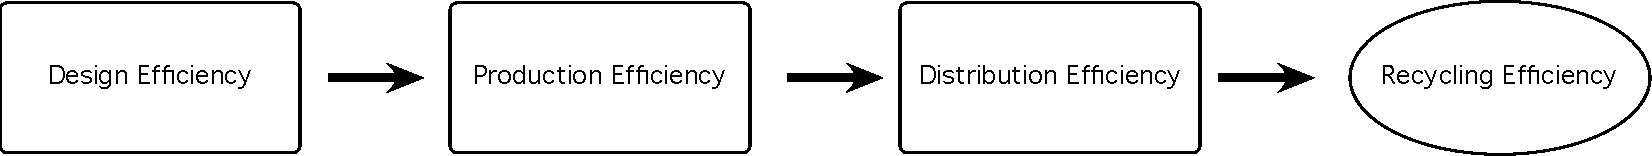
\includegraphics[width=\textwidth]{figures/system-process.pdf}
	\caption {Block-scheme of a system process.}
	\label{fig:systemProcess}
\end{figure}

Because we are talking about efficiency, we can consider the 
problem as a maximization of the production function $f_p$.
Table~\ref{tab:symbols} is a table of symbols and descriptions, as will
be used in the following explanations. It is important to note that not
all attributes will be covered in this text. The purpose of this essay
and the formulas suggested are done so to give a starting point for
calculation, highlighting the most relevant, overarching attributes for
consideration.

\begin{table}[h!]
	\begin{center}
%\begin{ruledtabular}
  \begin{tabular}{l c c}
\hline
\hline
		Logic Symbol & Description
\\
\hline
$E_\text{design}$ & Design efficiency
\\
$E_\text{p}$ & Production efficiency
\\
$E_\text{dist}$ & Distribution efficiency
\\
$E_\text{r}$ & Recycling efficiency
\\
$f_\text{p}$ & Production functional
\\
$E^i_\text{design}$ & Design efficiency standards
\\
$t_\text{d}$ & Durability
\\
$A_\text{design}$ & Adaptivity
\\
$g^1_\text{c}, g^2_\text{c}, \dots, g^{N_\text{c}}_\text{c}$ & Genre
components
\\
$N_\text{c}$ & Minimum number of genre components
\\
$H_\text{l}$ & Human labor
\\
$A_\text{l}$ & Automated labor
\\
$f_\text{design}$ & Design efficiency functional
\\
$D_\text{s}$ & Demand splitting value
\\
$\tilde{A}$ & Flexible automation process
\\
$\bar{A}$ & Fixed automation process
\\
$C_i$ & $i$th Consumer
\\
$D_i$ & $i$th Distributor
\\
$d_\text{p}$ & Distance to production facilities
\\
$d_\text{dist}$ & Distance to distribution facilities
\\
$P_\text{reg}$ & Regenerative protocol
\\
\hline
\hline
\end{tabular}
%\end{ruledtabular}
\end{center}
 \caption{\label{tab:symbols}Logic symbols and description.}
\end{table}


A full algorithmic calculation of this nature, taking into account all
related sub-processes in real life terms would require an enormous
text/programming treatment and will likely occur in a future edition of
this text's appendix, as an ongoing project development. 


\section {Collaborative Design Interface} 
The starting point for interaction in a NLRBE is the CDI, or
collaborative design interface. The CDI could abstractly be considered
the \textquote{new market} or the market of ideas or designs. Design is
the first step in any production interest and this interface can be
engaged by a single person; it can be engaged by a team; it can be
engaged by everyone. It is open source and open access and it would come
in the form of an online web interface.

The notion of \textquote{market} is expressed here not to conflate the
notion of trade, but rather the notion of sharing and group
decision-making. As with the traditional sales market, there is a swarm
type of behavior which makes decisions over time as a group whole with
respect to what goods will develop (demand) and what goods will perish
(lack of demand). In a certain sense, this democratic process is
embraced in a NLRBE, but by different means.

Moreover, all submitted designs, in creation or deemed complete, are
stored in an open access, searchable database. This database makes all
designs available for others to use or build upon. In this way, it is
similar to a traditional goods catalog commonly found today, except it
contains digital designs that can be sent into production at any time,
on demand.

This design creation and proposal system is how demand itself is
assessed. Instead of traditional advertising and the unidirectional
consumer good proposal system - where companies work to persuade the
consumer as to what they should buy, with the public mostly going with
the flow, favoring or not favoring a company's pitched good, component
or feature by purchase or not - this system works in an opposite, more
involved and democratic manner.

In this new, open source type design approach, the entire global
community has the option of presenting ideas for everyone to see,
weighing in on and building upon designs, harnessing the power of
collective experience and global knowledge.

The mechanism of the CDI would come in the form of an interactive
interface, such as we see commonly today with computer-aided design
(CAD) or computer-aided engineering (CAE) software. In short, these
programs are able to digitally create and represent any given product
design, containing all information as to how it should be made in final,
physical manufacturing.

\begin{figure}[bt!]
	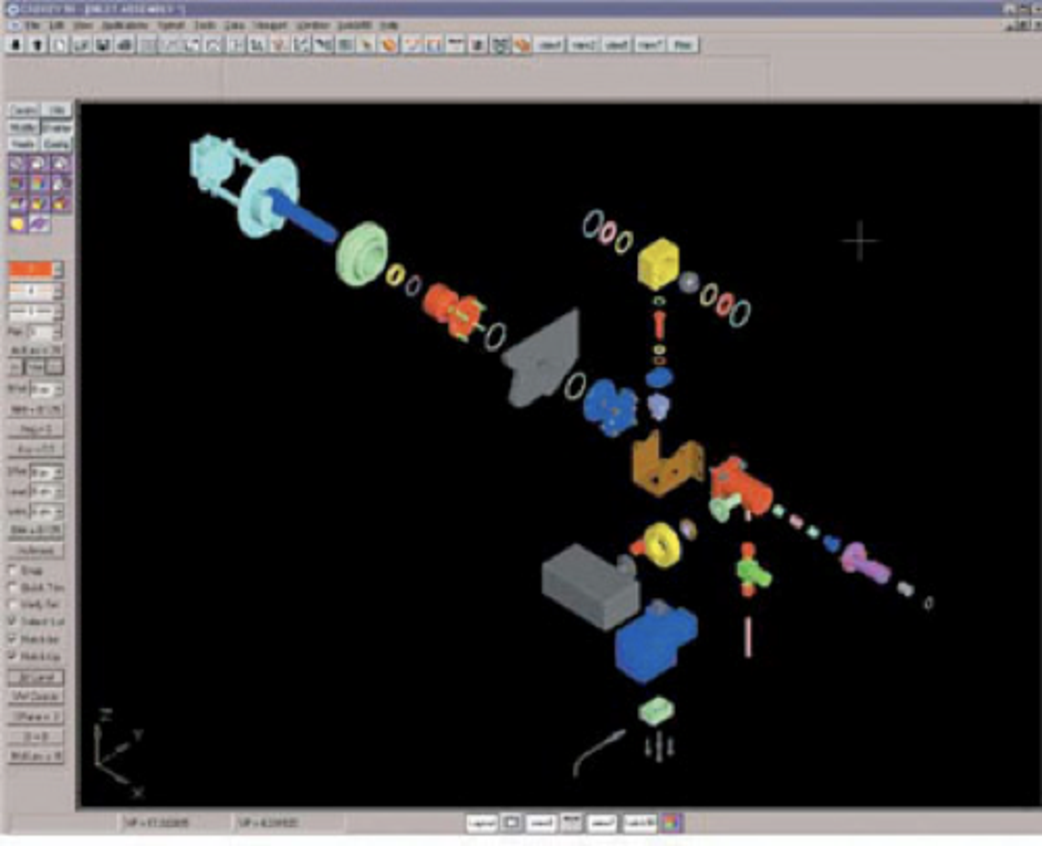
\includegraphics[width=\textwidth]{figures/CAD-design-example.pdf}
	\caption {CAD interface design example.}
	\label{fig:cadExample}
\end{figure}
 
As an aside, many considering the educational requirements to engage
such an interface, might be concerned about use-complexity. Naturally,
the more dedicated designer will develop the skills needed to whatever
degree interested while, for the more casual user, different degrees of
interface complexity and skill orientation can be utilized.

This more user-friendly interfacing can develop in a similar fashion to
how personal computers transitioned from complex proprietary coding
interfaces with manually input instructions, to the now ubiquitous,
simple graphic interface icon system, which allows users to operate more
intuitively. Future CAD/CAE type programs will likely evolve in the same
way, making the interactive process more accessible.

In many cases, as the database is always populated with current, already
existing designs, the practice will be to build upon other's work. For
example, if an engineer is interested in the optimization of a cell
phone, they have the option of building upon any existing phone product
design in the database, rather than starting from scratch.

The benefit of this cannot be emphasized enough as a collaborative
platform. Rather than limit the design input to, say, a boardroom of
engineers and marketers, as is common practice today, literally millions
of minds can be brought together to accelerate any given idea in this
approach. This new incentive system also ensures everyone interested in
the good will receive exactly what everyone else is likely to receive in
its advanced optimization states, where \emph{personal interest becomes
directly tied to societal interest}.

Also, given the patterns today, likely not everyone would want or need
to be a designer. Many people would be satisfied enough by what had been
set in motion already by others, with perhaps minor customization along
the way. Today, a very small percentage of the population actually
create and engineer the dominant technology and goods we use; and this
specialization may naturally continue in the future to some degree, even
though it is to the advantage of everyone if more minds came together.
If the educational system is orientated away from rote learning and its
antiquated basis that originated in the 19th century social order, we
could see an explosion of input and creativity.

All that understood, an incredibly important component of these design
and engineering programs today is how they can now incorporate advanced
physics and other real world, natural law properties with the proposed
design for testing. In other words, the good isn't just viewable in a
static visual model with noted properties, it can actually be tested
right there, virtually, to a relevant degree.

For instance, all new automobile designs today, long before they are
physically built, are run through complex digital testing processes that
assist in design integrity greatly~\cite{Keenan:http:95}. Over time,
there is no reason to believe that we will not be able to digitally
represent, and set in motion for testing, most all known laws of nature,
applying them in different contexts, virtually.

\section {Optimized Efficiency Standards}

Efficiency standards are standards by which a given design must conform.
This evaluation will be calculated automatically, or algorithmically, by
the CDS's programming. This can also be thought of as a \emph{filtering}
process.

In short, any proposed design will be digitally filtered through a
series of \emph{sustainability} and \emph{efficiency} protocols which
relate not only to the state of existing resources, but also to the
current performance of the total industrial system.  These would include
the following \textquote{efficiency standards}:\footnote{
	Please note these protocols were also addressed in the essay
	\emph{True Economic Factors}, in the context of
	\textquote{microeconomic components}, with mild variation in the
	language.
}
\begin{enumerate}
\item Strategically maximized durability
\item Strategically maximized adaptability
\item Strategic standardization of genre components
\item Strategically integrated recycling conduciveness
\item Strategic conduciveness for labor automation
\end{enumerate}
The Design efficiency 
\begin{equation}
	E_\text{design} = f_\text{design}(t_\text{d}, A_\text{design},
	c_\text{r}, N_\text{c}, H_\text{l})
	\label{eq:designEfficiency}
\end{equation}
is one of the main factors that can affect the overall efficiency of the
manufacturing and distribution process. This design efficiency depends
on several key factors $E^i_\text{design}$, which can be called \emph{current efficiency standards}. Here the index $i$ corresponds to some
particular standard.

Each standard will be generally explored as follows, expanding in
certain cases with respect to the symbolic logic associated, for the
sake of clarity. 

\begin{enumerate}
  \item 
  \textbf{Strategically Maximized Durability} means to make the good
  as strong and lasting as relevant. The materials utilized,
  comparatively assuming possible substitutions due to levels of scarcity
  or other factors, would be dynamically calculated, likely automatically
  by the design system, to be most conducive to an optimized durability
  standard.
  The maximization $t_\text{max}$ of the durability
  $t_\text{d}(d_1,\dots,d_n)$ can
  be considered as a local optimization issue. It can be analyzed by
  introducing the factors $d_i$ with $i\in[1,n]$, which affect it 
  $$
 		t_\text{max} = \max \;\; t_\text{d}(d_1,\dots,d_n) =
 		t_\text{d}(d^0_1,\dots,d^0_n),
  $$
  where the $d^0_i$ are some optimal values of the factors.

  \item
  \textbf{Strategically Maximized Adaptability} $A_\text{design}$
  means the highest state of flexibility for replacing component parts is
  made. In the event a component part of a good becomes defective or out
  of date, the design facilitates that such components are easily
  replaced to maximize full product life span, always avoiding the
  interest to replace the good as a whole.
 
  \item
  \textbf{Strategic Standardization of Genre Components} means all new designs either conform to or replace existing components
  $$
 	 g^1_\text{c}, g^2_\text{c}, \dots, g^{N_\text{c}}_\text{c}
  $$
  which are either already in existence or outdated due a lack of
  comparative efficiency. This logic should not only apply to a given
  product, it should apply to the entire good genre, however possible. 
 
  The aim is to minimize the total number of genre components
  $N_\text{c}$. In other words, the standardization of the process will
  enable the possibility of lowering the number $N_\text{c}$ to a
  possible minimum and thus reduce the number of needed genre components
  $g_\text{c}$.

	\item
	\textbf{Recycling Conduciveness} $c_\text{r}$ means every design must
	conform to the current state of regenerative possibility. The
	breakdown of any good must be anticipated in the initial design and
	allowed for in the most optimized way.

	\item 
	\textbf{Strategic Conduciveness for Labor Automation} means that the
	current state of optimized, automated production is also taken into
	account, seeking to refine the design to be most conducive to
	production with the least amount of complexity, human labor or
	monitoring. Again, we seek to simplify the way materials and
	production means are used so that the maximum number of goods can be
	produced with the least variation of materials and production
	equipment. 

	This is denoted by human labor $H_\text{l}$ and automated labor
	$A_\text{l}$. The aim is to minimize the human interaction with the
	production process. This can be written as: 
	$$
		\frac{H_\text{l}}{H_\text{l} + A_\text{l}} \rightarrow \min
	$$
  Using this equation, we could also write a simpler condition: 
	$$
		\frac{H_\text{l}(l_1,\dots,l_n)}{A_\text{l}(l_1,\dots,l_n)}
		\rightarrow \min,
	$$ 
  where are factors that influence human and automatic labor. 
\end{enumerate}

So, returning to equation~\eqref{eq:designEfficiency}, the
\textquote{Optimized Design Efficiency} function can be described by a
function $f_\text{design}$, where $t_\text{d}$ is durability,
$A_\text{design}$ is adaptability, $c_\text{r}$ is recycling
conduciveness, $N_\text{c}$ is the minimum number of genre components
and $H_\text{l}$ is a human labor. 

\section {The Industrial Network}

The industrial network refers to the basic network of physical
facilities that are directly connected to the design and database system
just described. The system connects servers, production facilities,
distribution facilities and recycling facilities, see
figure~\ref{fig:industrialNetwork}.

\begin{figure}[bt!]
	\centering
	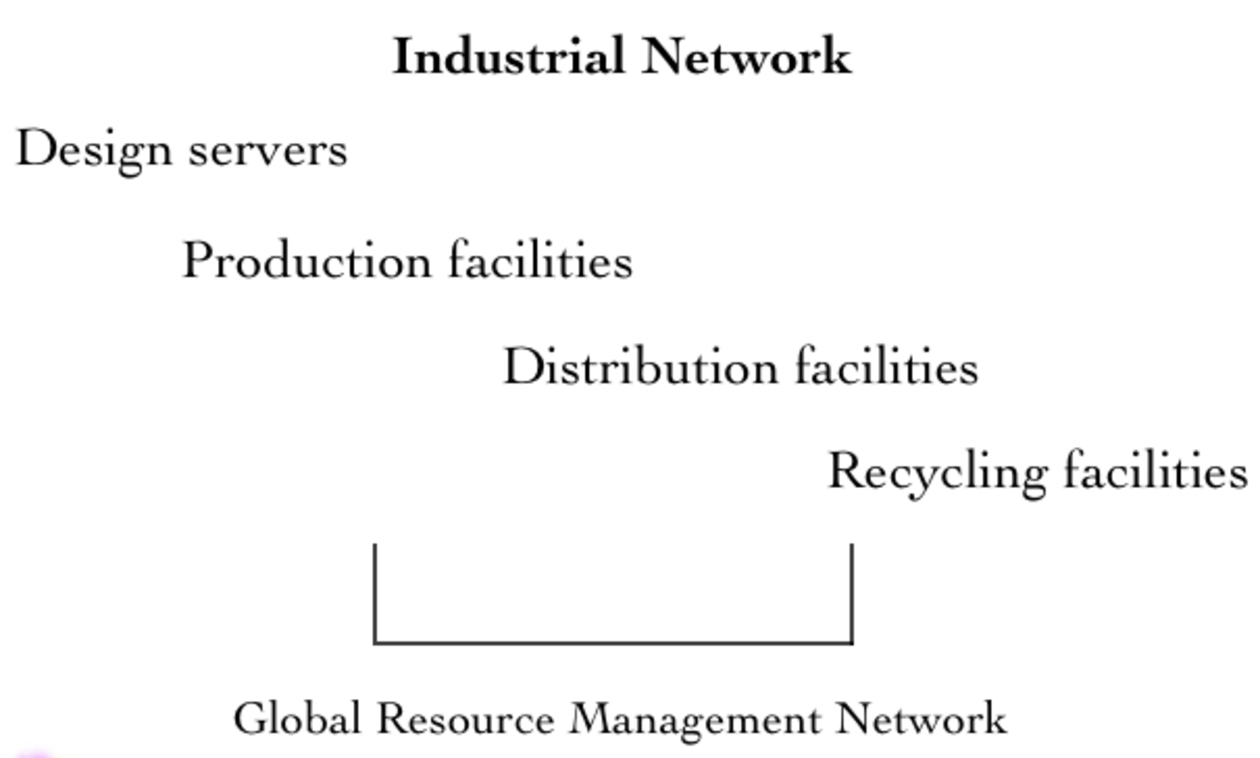
\includegraphics[width=0.75\textwidth]{figures/industrial-network.pdf}
	\caption {Industrial Network visual aid.}
	\label{fig:industrialNetwork}
\end{figure}

\subsection {Design Servers}

These computer servers connect the design database to the
designers/consumers, while constantly being updated with relevant
physical data to guide the process of product creation in the most
optimized and sustainable way. 

As noted, the engaged CDI (or collaborative design interface) is an open
source program that facilitates collective, computer-aided design,
running each step through the set of efficiency and sustainability
filters [i.e. equation~\eqref{eq:designEfficiency}] which assure
optimized design. These designs are tested in real time, digitally, and
in most cases, the good will exist in whatever state online for others
to obtain, on demand, or for use as a preliminary model by which new
ideas can be built upon. 


\subsection {Production Facilities}

These structures facilitate the actual manufacturing of a given design.
These would evolve as automated factories that increasingly are able to
produce more with fewer material inputs and fewer machine
configurations. Again, if the interest existed to consciously overcome
unnecessary design complexities, we can further this efficiency trend
with an ever-lower environmental impact and ever lower resource use per
task, while maximizing our abundance producing potential. 

The number of production facilities, whether homogeneous or
heterogeneous, would be strategically distributed topographically based
on population statistics, no different than how grocery stores today try
to average distances between pockets of people around neighborhoods.
This is the \textquote{proximity strategy} which will be revisited in
this essay. 


\subsection {Distribution Facilities}

Distribution can either occur directly from the production facility,
usually in the case of an on-demand, one-off production for custom use,
or sent to a distribution \emph{library} for public access in masse,
based on regional demand interest. 

Some goods will be conducive to low demand, custom production and some
will not. Food is the easiest example of a mass production necessity,
while a personally tailored piece of furniture would come directly from
the manufacturing facility once created. 

It is worth reiterating that regardless of whether the good is
classified to go to a library or directly to a user, this is still an
'access system'. In other words, at any time, the user of the custom or
mass produced good can return the item for reprocessing or restocking. 


\subsection {Recycling Facilities}

Recycling Facilities would likely exist as part of the production
facility, allowing access to returned parts for updating and
reprocessing. As noted in the design protocol, all goods have been
pre-optimized for 'conducive recycling'. The goal here is a zero-waste
economy. Whether it is a phone, a couch, a computer, a jacket, or a
book, everything goes back to a recycling facility, likely the point of
origin, which will directly reprocess any item as best it can. 

Of course, an item may be returned elsewhere if needed; the integrated
and standardized production and recycling centers, having been conceived
of as a complete, compatible and holistic system, would be able to
handle returned goods optimally, as is not the case today. 


\subsection {Global Resource and System Management}

These four facilities are also connected, to one degree or another, to a
\emph{Global Resource Management } (GRM) network, which is a sensor and
measurement system that provides feedback and information about the
current state of raw materials and the environment. 

\section {Resource Management, Feedback and Value}

As noted, this computer-aided design and engineering process does not
exist in a vacuum; it does not process designs with no input as to the
current state of the planet and its resources. Connected to the design
process, literally built into the noted \textquote{Optimize Design Efficiency} function, is dynamic feedback from an Earth-wide accounting system that gives data about all relevant resources which pertain to all productions. 

To whatever degree technically possible, all raw materials and related
resources are tracked and monitored, in as close to real time as
possible. This is mainly because maintaining equilibrium with the
Earth's regenerative processes, while also working strategically to
maximize the use of the most abundant materials, while minimizing
anything with emerging scarcity, is a critical efficiency calculation.
Again, this is, in part, the purpose of the Global Resource Management
system mentioned prior. 

As far as \textquote{value} calculation, perhaps the two most important measures, which will undergo constant dynamic recalculation through feedback as industry unfolds, is the level of (a) 'scarcity' and the degree of (b) 'labor complexity'. 

\subsection {Scarcity value}
'Scarcity value' can be assigned a numerical value, from 1-100. 1 would
denote the most severe scarcity with respect to the current rate of use
and 100 the least severe. 50 would be the steady-state dividing line,
see figure~\ref{fig:scarcity}.  The scarcity value of any given resource
would exist at some value along this line, dynamically updated by the
Global Resource Management network. 
	
\begin{figure}[bt!]
	\centering
	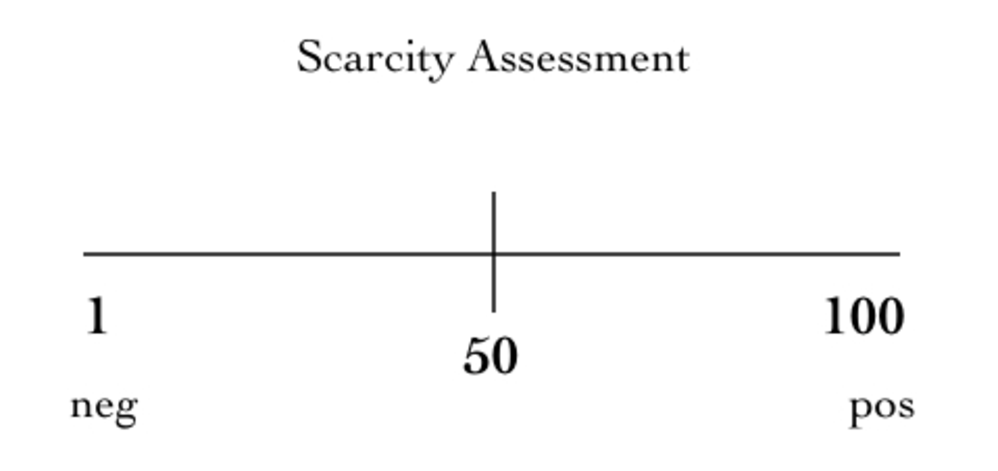
\includegraphics[width=0.6\textwidth]{figures/scarcity.pdf}
	\caption {Scarcity rank visual aid.}
	\label{fig:scarcity}
\end{figure}

For example, if the use of wood passes the steady state level of 50,
which would mean consumption is currently surpassing the Earth's natural
regeneration rate, this would trigger a counter move of some kind, such
as the process of 'material substitution' or finding a replacement for
wood in any future productions. 

As far as a comparative evaluation, in a market system the price
mechanism is used to decide which material is more cost efficient,
assuming a given price will have already accounted for relevant
technical information or, in this case, the issue of scarcity.

This new approach, rather than use price to compare or assess value,
accounts for a given technical quality directly by a comparative
quantification. In the case of scarcity concerns, it is best to organize
genres or groups of similar use materials and quantify, to the highest
degree possible, their related properties and degrees of efficiency for
any given purpose. Then, a general numerical value spectrum is applied
to those relationships. 

For example, there is a spectrum of metals that have different
efficiencies for electrical conductivity. These efficiencies can be
physically quantified and then compared by value. So, if copper, a
conductive metal, goes below the 50 value of equilibrium regarding its
scarcity, calculations are triggered by the management program to
compare the state of other conducive materials, their \emph{scarcity
level} and their \emph{efficiency level}, preparing for substitution. 

This is just one example and naturally this type of reasoning would get
extremely complicated depending on the material and purpose problems
posed. However, that is exactly why it is calculated by machine, not
people. The human mind, either singly or organized into large groups,
simply cannot process such data effectively. Also, it is worth pointing
out that this type of direct value calculation, based around purpose,
conduciveness and sustainability, dramatically eclipses the price
mechanism when it comes to true resource awareness and intelligent
resource management in calculation. 

\subsection {Labor complexity}

Likewise, 'labor complexity' and its assessment simply means estimating
the complexity of a given production and drawing a numerical value based
on the degree of process complexity. Complexity, in the context of an
automation-oriented industry, can be quantified by defining and
comparing the number of 'process stages'. Any given good production can
be foreshadowed as to how many 'stages' of production processing it will
take. It can then be compared to other good productions, ideally in the
same purpose genre, for a quantifiable assessment. In other words, the
units of measurement are these 'stages'.

For example, a chair that can be molded in three minutes, from simple
polymers in one process, will have a lower 'labor complexity' value than
a chair which requires automated assembly down a more tedious production
chain, with mixed materials. In the event a given process value is too
complex or hence comparatively inefficient in terms of what is currently
possible (by comparison to an already existing design of a similar
nature), the design would be flagged and would hence need to be
re-evaluated. 

Such adjustments and flagging would come in the form of feedback from
the design interface, during the design stage. There is also no reason
not to assume that with ongoing advancement in AI, the system could
actually feed back with actual suggestions or even direct solutions to a
given efficiency or sustainability problem, in real time. 

\section {Design Calculation}

Those generalizations noted, a walkthrough of this overall, linear
process is expressed below. There will be some repetition here for the
sake of clarity. If we were to look at good design in the broadest
possible way with respect to industrial unfolding, we end up with about
four functions or processes, each relating to the four dominant, linear
stages, including design, production, distribution and recycling. Again,
each of these processes is directly tied to the Global Resource
Management system that provides value feedback that assists in the
regulatory apparatus to ensure efficiency and sustainability. 

The following propositions apply, \new{see
equation~\eqref{eq:designEfficiency}}:
$
	E_\text{design} = f_\text{design}(t_\text{d}, A_\text{design},
	c_\text{r}, N_\text{c}, H_\text{l})
$
All Product Designs must adapt to: 
\begin{enumerate}
  \item  Optimized Design Efficiency 
  \item  Optimized Production Efficiency 
  \item  Optimized Distribution Efficiency 
  \item  Optimized Recycling Efficiency 
\end{enumerate}

\subsection {Optimized Design Efficiency}
A product design must meet or adapt to criteria set by current
efficiency standards $E_\text{design}$. The current efficiency standards
have five evaluative sub-processes, as expressed before: 
\begin{itemize}
 \item Durability $t_\text{d}$
 \item Adaptability $A_\text{design}$
 \item Standardization \new{with minimum number of genre components} $N_\text{c}$ 
 \item Recycling Conduciveness $c_\text{r}$
 \item Automation Conduciveness $H_\text{l}$ \bs{shouldn't it be
 $A_\text{l}$ here?} 
\end{itemize}

Please note that further breakdown of each of these sub-processes and
logical associations can be figuratively made as well to ever-reducing
minutiae. However, as noted, this expression is the \textquote{top} tier
by which all other sub-processes are oriented. It is, again, not the
scope of this text to provide all attributes of a working algorithm. It
is also not implied here that the parameters expressed are total or
absolutely complete.

\subsection {Optimized Production Efficiency}

\new{The parameters of the optimized production efficiency filter, see
blue box in figure~\ref{fig:classDeterminationProcess},} can
change based on the nature of the facilities and how much machine
variation in production (fixed automation vs. flexible
automation)\footnote{
	"Fixed automation", also known as \textquote{hard automation}, refers
	to an automated production facility in which the sequence of
	processing operations is fixed by the equipment configuration. It is
	fast but has less variation in output design capacity. Flexible
	automation can create more variation but the disadvantage is the time
	required to reprogram and change over the production equipment. These
	terms are common to the manufacturing and robotics industry when it
	comes to plant design.
}
is required at a given time. For the purpose of expression, two facility
types will be distinguished: one for high demand or mass production and
one for low demand or short-run, custom goods. Very simply, a class
determination is made\new{, see blue box in
figure~\ref{fig:classDeterminationProcess},} which splits the destination facilities based upon
the nature of production requirements \new{$D$ and a threshold demand
$D_\text{s}$ at which is decided for the product to either run in high
demand/mass production ($D > D_\text{s}$) or low demand/custom
production ($D < D_\text{s}$)}.
The 'high demand' target\new{, left branch in
figure~\ref{fig:classDeterminationProcess},} assumes fixed automation $\bar{A}(a_i)$,
meaning unvaried production methods ideal for high demand/mass
production. The 'low demand' target\new{, right branch in
figure~\ref{fig:classDeterminationProcess},} uses flexible automation
$\tilde{A}(t,D_c(t),a_i)$, which can do a variety of things but usually
in shorter runs. \bs{What is $t$, time? What is $D_c$? $D_i$ was defined
as the $i$th distributor. What are the $a_i$?}

\begin{figure}[bt!]
	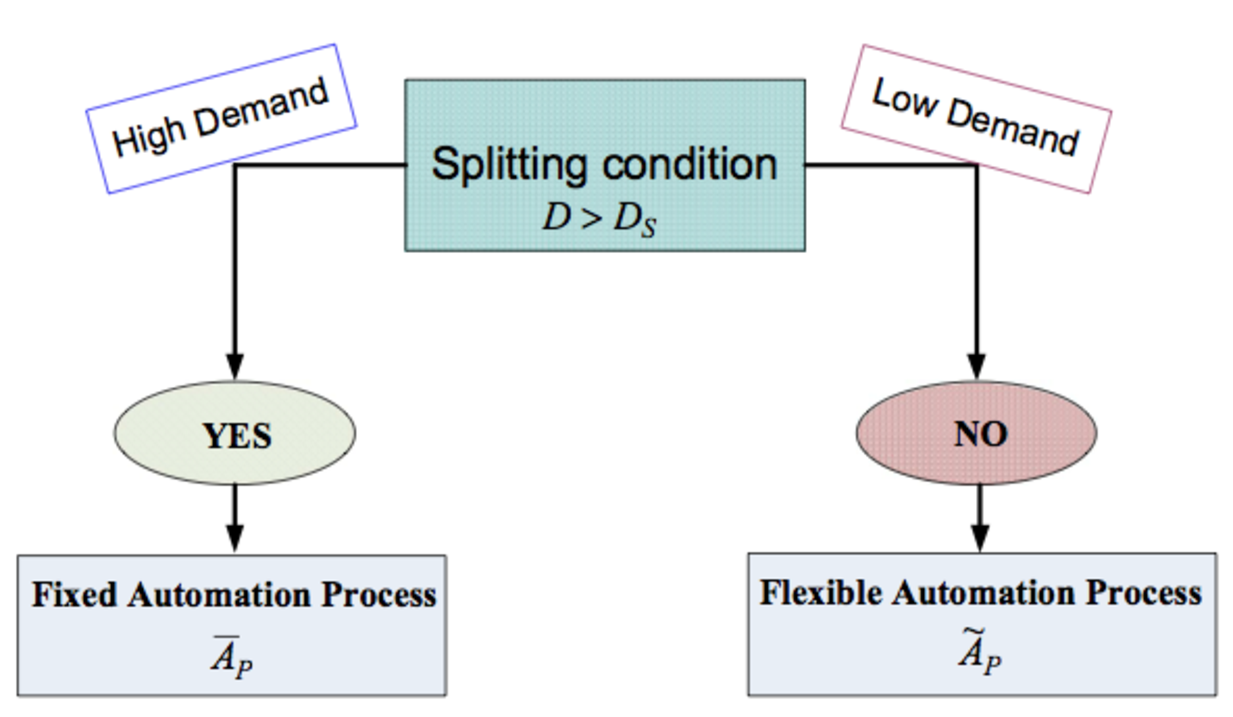
\includegraphics[width=\textwidth]{figures/class-determination-process.pdf}
	\caption{Dividing by low and high. Application of the class determination process.}
	\label{fig:classDeterminationProcess}
\end{figure}

Again, this schematic assumes only two types of facilities are needed.
There could be more facility types based upon production factors,
generating more splitting conditions. However, if the design rules are
respected, there shouldn't be too much variation over time as the intent
is always to reduce and simplify.

To state the process in linear form, see
figure~\ref{fig:classDeterminationProcess}:
All product designs are filtered by a [Demand Class Determination]
process. The [Demand Class Determination] process filters based on the
standards set for [Low Demand] or [High Demand]. All [Low Consumer
Demand] product designs are to be manufactured by the [Flexible
Automation] process. All [High Consumer Demand] product designs are to
be manufactured by the [Fixed Automation] process. Also, both the
manufacturing of [Low Consumer Demand] and [High Consumer Demand]
product designs will be regionally allocated as per the [Proximity
Strategy] $d_\text{p}$ of the manufacturing facilities.

\subsection {Optimized Distribution Efficiency}

Once process 2 is finished, the product design becomes a 'product' and
moves to the [Optimized Distribution Efficiency] filter. In short, all
products are allocated based on its prior [Demand Class Determination].
[Low Consumer Demand] products follow the [Direct Distribution] process.
[High Consumer Demand] productions follow the [Mass Distribution]
process, which would likely be the libraries, mentioned prior. Both the
[Low Consumer Demand] and [High Consumer Demand] product will be
regionally allocated as per the [Proximity Strategy], as before. 

In the case of [Low Consumer Demand] $D_\text{c} < D_\text{s}$ the
distribution scheme is direct, see figure~\ref{fig:distributionSchemes}
(left). In this case the product goes directly to the consumer without
the help of network intermediaries.

\begin{figure}[bt!]
	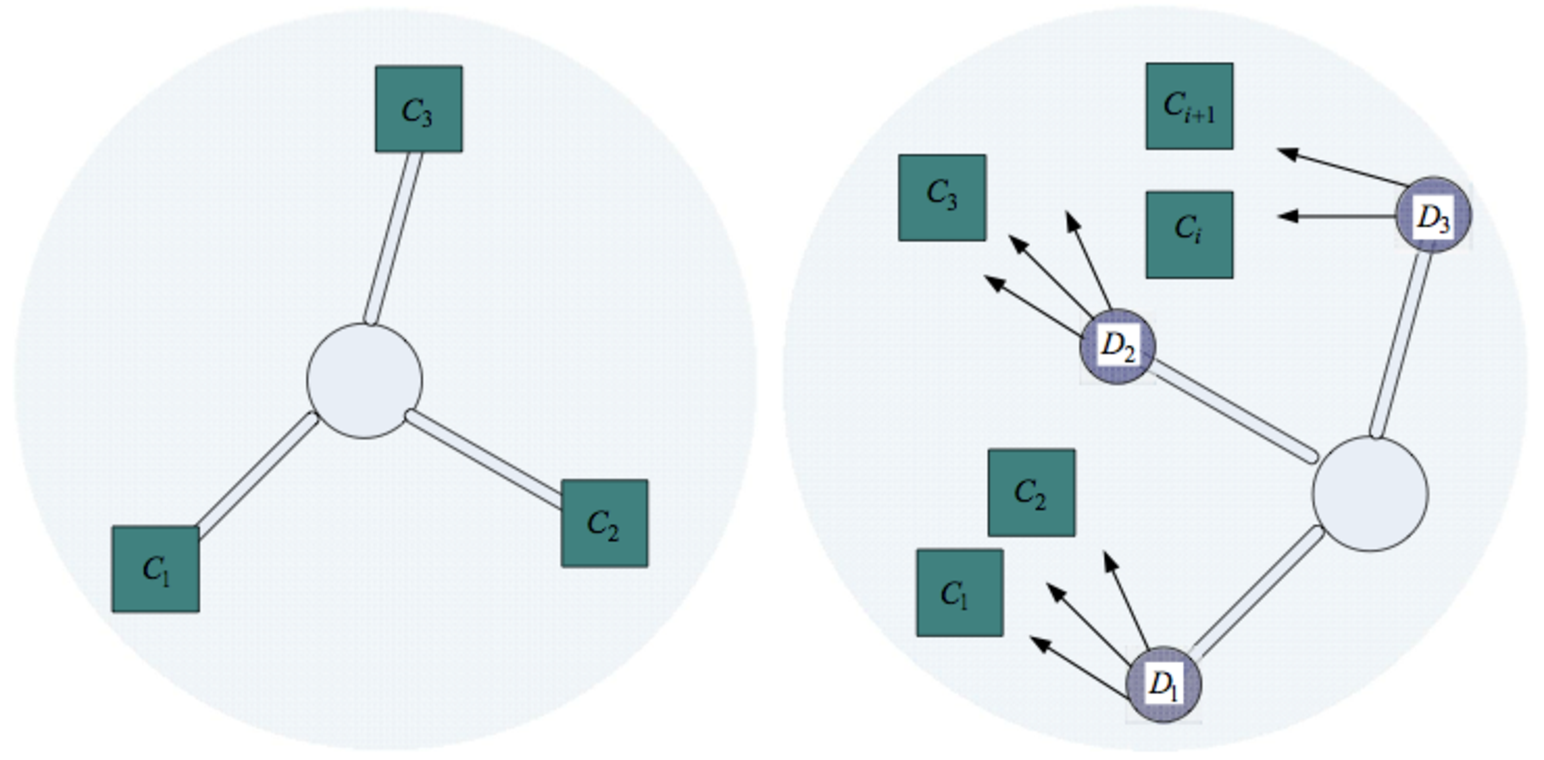
\includegraphics[width=\textwidth]{figures/distribution-schemes.pdf}
	\caption[Distribution schemes]{Illustration of distribution schemes.
	(left) Direct distribution for low demand case. (right) Mass
	distribution for high demand case.}
	\label{fig:distributionSchemes}
\end{figure}

In the case of [High Consumer Demand] $D_\text{c} > D_\text{s}$ the
distribution scheme is mass, see figure~\ref{fig:distributionSchemes}.
In this case the product goes to intermediary \new{distribution}
facilities $D_i$, such as libraries, to engage the potential consumers
$C_i$. 

Similar to the production efficiency considerations, in the case of
'Distribution Efficiency' $E_\text{dist}$,\bs{Why different emphasis
styles? Brackets vs single quotes vs \emph{italics}?} for the low and
high demand, the distribution process will be optimized in terms of the
distance $d_\text{dist}$ to the existing facilities.  In this case the
facilities are places in regional distribution (libraries), based on the
level of demand in the given region, i.e.  proximity strategy
$d_\text{p}$. 

\subsection {Optimized Recycling Efficiency}

After distribution, the product then goes through its life-cycle. Once
its life-cycle ends, the product becomes \textquote{void} and moves to
process 4, or the [Optimized Recycling Efficiency] filter. In short,
all voided products will follow the current [Regenerative Protocol]
$P_\text{reg}$. This protocol embraces the standards employed at that
time to ensure the optimized reuse or reincorporation of any given good
or component. Naturally, the sub-processes of this are vast and complex
and it is the role of engineers, embracing natural law physics, to best
understand exactly what parameters will be set.


\chapter {Lifestyle, Freedom and The Humanity Factor}


\part {The Zeitgeist Movement \label{part:zeitgeistMovement}}
\chapter {Social Destabilization and Transition}
\chapter {Becoming The Zeitgeist Movement}

\part {Appendix}
\chapter {Vocabulary List (pending)}
\chapter {The Scientific Method (pending)}
\chapter {Reading List (pending)}
\chapter {ZM: Structure and Processes (pending)}


%%%%%%%%%%%%%%%%%%%%
%%% bibliography %%%
%%%%%%%%%%%%%%%%%%%%
\bibliographystyle{alpha}
\bibliography{tzm}

\end{document}
